\clearpage

\onecolumn
\aistatstitle{SNAP: Sequential Non-Ancestor Pruning for Targeted Causal Effect Estimation With an Unknown Graph \\
Supplementary Materials}

\section{ORIENTING V-STRUCTURES}
\label{app:vstruct}

Algorithms~\ref{alg:pc-v} and \ref{alg:rfci-v} correspond to orienting v-structures as done in the PC algorithm \citep{spirtes2000causation} and the RFCI algorithm \citep{colombo2012learning} algorithms. Both algorithms use the meta-symbol $*$ as a wildcard to denote both edge tails and arrowheads. This allows edges to be oriented as bi-directed. Bi-directed edges indicate \emph{conflicting v-structures} that arise when performing \ac{CI} tests only up to some order $k$ \citep{wienobst2020recovering}. Fig.~\ref{fig:bidirected_cpdag} shows an example for how a bidirected edge can arise when performing \ac{CI} tests up to order 0.

Lemma~\ref{lem:vstructure} describes the conditions for correctly orienting v-structures.
In particular, the dependency conditions  $X \dep Z | sepset(X,Y)$ and $Z \dep Y | sepset(X,Y)$ are the same as in Lemma~3.1 by \citet{colombo2012learning}.
Thus, we adopt Algorithm~4.4 in \citep{colombo2012learning} to orient v-structures, as shown by Algorithm~\ref{alg:rfci-v}.
Fig.~\ref{fig:rfci_example} shows an example where PC-style v-structure orientations, as given by Algorithm~\ref{alg:pc-v}, would orient an edge bidirected, even though the edge exists in the true CPDAG.

\begin{algorithm}
\centering
\caption{OrientVstructPC: Orienting v-structures in the PC algorithm \citep{spirtes2000causation}}
\label{alg:pc-v}
\begin{algorithmic}[1]
    \Require Skeleton $\hat{U}$, separating sets $sepset$
    \State$\hat{G} \gets \hat{U}$
    \For{$X - Z - Y$ in $\hat{\mathbf{E}}$ such that $X \notin Adj_{\hat{U}}(Y)$}
        \If{$Z \notin sepset(X,Y)$}
            \State Orient $X \starleft-\starright Z \starleft-\starright Y$ as $X \starleft\to Z \gets\starright Y$ in $\hat{G}$
        \EndIf
    \EndFor
\State\Return{$\hat{G}$}
\end{algorithmic}
\end{algorithm}



\begin{algorithm}
\centering
\caption{OrientVstructRFCI: Orienting v-structures in the RFCI algorithm \citep{colombo2012learning}}
\label{alg:rfci-v}
\begin{algorithmic}[1]
    \Require Skeleton $\hat{U}$, separating sets $sepset$
    \State $M \gets \{(X,Z,Y) \text{ such that } X - Z - Y$ in $\hat{\mathbf{E}}$ \text{ and } $X \notin Adj_{\hat{U}}(Y)\}$
    \State $L \gets \{\}$
    \Repeat
        \State $X,Z,Y \gets$ choose an unshielded triple from $M$
        \If{$Z \notin sepset(X,Y)$}
            \If{$X \dep Z | sepset(X,Y)$ and $Z \dep Y | sepset(X,Y)$}
                \State $L \gets L \cup \{(X,Y,Z)\}$ \Comment{Add to legitimate v-structures}
            \Else
                \For{$V \in \{X,Y\}$}
                    \If{$V \indep Z | sepset(X,Y)$}
                        \State $\mathbf{S} \gets sepset(X,Y)$
                        \Comment{Find minimal separating set}
                        \State done $\gets$ False
                        \While{not done}
                            \State done $\gets$ True
                            \For{$S \in \mathbf{S}$}
                                \If{$V \indep Z | \mathbf{S} \setminus \{S\}$}
                                    \State $\mathbf{S} \gets \mathbf{S} \setminus \{S\}$
                                    \State done $\gets$ False
                                    \State \textbf{break}
                                \EndIf
                            \EndFor
                        \EndWhile
                        \State $sepset(V,Z) \gets sepset(Z,V) \gets \mathbf{S}$
                        \State $M \gets M \cup$ all triangles $(\min(V,Z),\cdot,\max(V,Z))$ in $\hat{U}$ \Comment{Update new unshielded triples.}
                        \State $M \gets M \setminus$ all triples in $M$ of the form $(V,Z,\cdot), (Z,V,\cdot), (\cdot,V,Z)$ and $(\cdot,Z,V)$
                        \State $L \gets L \setminus$ all triples in $L$ of the form $(V,Z,\cdot), (Z,V,\cdot), (\cdot,V,Z)$ and $(\cdot,Z,V)$
                        \State Delete the edge $V - Z$ from $\hat{U}$
                    \EndIf
                \EndFor
            \EndIf
        \EndIf
    \Until{$M$ is empty}
    \State$\hat{G} \gets \hat{U}$
    \For{$(X, Z, Y) \in L$}
        \State Orient $X \starleft-\starright Z \starleft-\starright Y$ as $X \starleft\to Z \gets\starright Y$ in $\hat{G}$
    \EndFor
\State\Return{$\hat{G}, sepset$}
\end{algorithmic}
\end{algorithm}

\begin{figure}[ht!]
    \centering
    \begin{subfigure}[b]{0.49\linewidth}
    \centering
    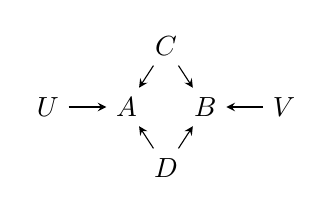
\begin{tikzpicture}[xscale = 1,yscale = 1.1]
        \node (a) at (0,0) {$A$};
        \node (b) at (1,0) {$B$};
        \node (c) at (0.5, 0.7) {$C$}
          edge [-stealth] (a)
          edge [-stealth] (b);
        \node (d) at (0.5, -0.7) {$D$}
          edge [-stealth] (a)
          edge [-stealth] (b);
        \node (u) at (-1,0) {$U$}
          edge [-stealth] (a);
        \node (v) at (2,0) {$V$}
          edge [-stealth] (b);
    \end{tikzpicture}
    \caption{Underlying true DAG}
    \label{fig:bidirected_dag}
    \end{subfigure}
    \begin{subfigure}[b]{0.49\linewidth}
    \centering
    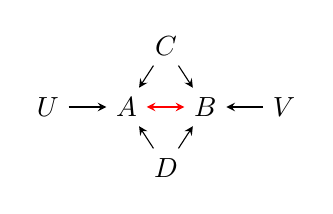
\begin{tikzpicture}[xscale = 1,yscale = 1.1]
        \node (a) at (0,0) {$A$};
        \node (b) at (1,0) {$B$}
          edge [stealth-stealth, red] (a);
        \node (c) at (0.5, 0.7) {$C$}
          edge [-stealth] (a)
          edge [-stealth] (b);
        \node (d) at (0.5, -0.7) {$D$}
          edge [-stealth] (a)
          edge [-stealth] (b);
        \node (u) at (-1,0) {$U$}
          edge [-stealth] (a);
        \node (v) at (2,0) {$V$}
          edge [-stealth] (b);
    \end{tikzpicture}
    \caption{Partially directed graph $G^0$ found by SNAP}
    \label{fig:bidirected_cpdag}
    \end{subfigure}
  \caption{Example of a bidirected edge, based on Figure 2 in \citep{wienobst2020recovering}. Fig.~\ref{fig:bidirected_dag} shows the underlying true DAG. Fig.~\ref{fig:bidirected_cpdag} shows the partially directed graph $G^0$ found by SNAP (with any targets) at iteration $i=0$ after performing only marginal \ac{CI} tests. Nodes $A$ and $B$ are not separated by the empty set, thus there is still an edge between them. This results in two conflicting v-structures, $U \to A \gets B$ and $A \to B \gets V$, indicated by the bidirected edge $A \leftrightarrow B$. As shown by \citet{wienobst2020recovering}, given low-order \ac{CI} tests, nodes with such a bidirected edge between them are not adjacent in the true CPDAG.}
  \label{fig:bidirected_example}
\end{figure}

% \clearpage
\section{PROOFS}
\label{app:proof}

\subsection{Proof for Lemma~\ref{thm:ancestors}}\label{app:ancestors}

\lemmaancestors*

\begin{proof}
    \citet{lauritzen1996graphical} (Proposition 3.22) and \citet{guo2023variable} (Lemma D.1) show that this holds for true causal graphs $D$ and ancestral sets.
    If two causal graphs are equal, then their \acp{CPDAG} are also equal.
    Since we assume that $\mathbf{V}^*$ is possibly ancestral (defined in Theorem.~\ref{thm:ancestors}), i.e., it contains all its own possible ancestors $PossAn_G(\mathbf{V^*}) \subseteq \mathbf{V^*}$, this implies that it also contains all its (actual) ancestors in the (unknown) ground truth DAG $D$. Hence, $\mathbf{V^*}$ is  ancestral in the unknown ground truth graph $D$, i.e. $An_D(\mathbf{V^*}) \subseteq \mathbf{V^*}$, in the MEC represented by the CPDAG $G$.
\end{proof}

\subsection{Proof for Theorem~\ref{thm:snap_is_sound}} \label{proof:snap_is_sound}

Theorem~\ref{thm:snap_is_sound} states that at each iteration $i$ of the SNAP(k) algorithm (Algorithm~\ref{alg:snap(k)}), the set of considered nodes $\hat{\mathbf{V}}^{i}$ contains all possible ancestors of the targets $\mathbf{T}$.
Additionally, $\hat{\mathbf{V}}^{i}$ is possibly ancestral, which means that it contains all of its own possible ancestors in the CPDAG $G$, i.e. $PossAn_G(\hat{\mathbf{V}}^{i}) \subseteq \hat{\mathbf{V}}^{i}$.  

To prove this result, we first show that no edge between the nodes $\hat{\mathbf{V}}^{i}$ are wrongly deleted during the execution of SNAP(k).
In other words, the intermediate undirected graph $\hat{U}^i$ over the subset $\hat{\mathbf{V}}^{i} \subseteq \mathbf{V}$ is a supergraph of $U|_{\hat{\mathbf{V}}^{i}}$, the induced subgraph of the true skeleton $U$ over $\hat{\mathbf{V}}^{i}$, at each iteration $i$. This means that  $\hat{U}^i$ contains all edges in $U|_{\hat{\mathbf{V}}^{i}}$, and possibly some additional edges.

\begin{lemma}
\label{lem:skeleton}
Given oracle conditional independence tests, at any iteration $i = 0,..,k$ of Algorithm~\ref{alg:snap(k)}, the undirected graph $\hat{U}^{i}$ is a supergraph of $U|_{\hat{\mathbf{V}}^{i}}$, the induced subgraph of the true skeleton $U$ over $\hat{\mathbf{V}}^{i}$.

\begin{proof}
In the Algorithm~\ref{alg:snap(k)} we only remove edges in $\hat{U}^i$ between two nodes $X, Y \in \hat{\mathbf{V}}^{i}$ for which we can find a separating set.
By faithfulness, we assume that these nodes are therefore also non-adjacent in the ground truth skeleton $U$.
Hence, the resulting skeleton $\hat{U}^i$ over the variables $\hat{\mathbf{V}}^{i}$ is a supergraph of the induced subgraph of the true skeleton, denoted by  $U|_{\hat{\mathbf{V}}^{i}}$.
\end{proof}

\end{lemma}

Next, we show that no possible ancestor of any target in $\mathbf{T}$ gets wrongly eliminated at any iteration $i$ of SNAP(k).
We first show that if we used the rules to orient v-structures from RFCI, described in Algorithm~\ref{alg:rfci-v}, for all iterations, this would hold.
We then prove that these rules are not necessary for $i=0,1$, but we can instead just use the standard rules for orienting v-structures in PC, described in Algorithm~\ref{alg:pc-v}.

% LEMMA B.2
\begin{lemma}
\label{lem:vstructure1}
Let $G$ be the CPDAG of the ground truth DAG $D$ and $\mathbf{T} \subseteq \mathbf{V}$ a set of targets.
Given oracle conditional independence tests, at any iteration $i = 0,..,k$ of SNAP (k) (Algorithm~\ref{alg:snap(k)}), let $\hat{U}^i$ be the undirected graph with nodes $\hat{\mathbf{V}}^{i}$ estimated at iteration $i$ and $\hat{G}^i$ be an initially undirected graph with the same skeleton. After orienting v-structures in $\hat{G}^i$ using the RFCI orientation rules, described in Algorithm~\ref{alg:rfci-v}, in SNAP(k) we collect in $\hat{\mathbf{V}}^{i+1}$ only the nodes $V \in \hat{\mathbf{V}}^{i}$ that have a possibly directed path to any $T \in \mathbf{T}$.
Then it holds that $PossAn_G(\mathbf{T}) \subseteq \hat{\mathbf{V}}^{i+1}$ and that $\hat{\mathbf{V}}^{i+1}$ is \emph{possibly ancestral}, i.e.,  
for all $V \in \hat{\mathbf{V}}^{i+1}$ it holds that $PossAn_G(V) \subseteq \hat{\mathbf{V}}^{i+1}$.

\end{lemma}
\begin{proof}
As shown in Lemma~\ref{lem:skeleton}, given oracle conditional independence tests at any iteration $i$ at Line 17 the skeleton $\hat{U}^i$ is a supergraph of the true skeleton $U$ restricted to the variables $\hat{\mathbf{V}}^{i}$.
We will now need to prove that orienting v-structures following the additional criteria in Algorithm~\ref{alg:rfci-v}, the orientations that we create in $\hat{G}^i$ are not in conflict with any possible ancestor of the variables $\hat{\mathbf{V}}^i$ in the ground truth CPDAG $G$. Our proof by contradiction follows the proof of Lemma~2 in \cite{wienobst2020recovering}. 

Let us assume that for an unshielded triple  $X \starleft-\starright Z \starleft-\starright Y$, the following three conditions hold: $Z \notin sepset(X,Y)$, $X \dep Z | sepset(X,Y)$ and $Z \dep Y | sepset(X,Y)$. Let us assume additionally that
$Z \in PossAn_G(X)$.
Then, there exists some DAG $D'$ in the \ac{MEC} represented by $G$ for which $Z \in An_{D'}(X)$. This means that there is a directed path from $Z \to \dots \to X$ in $D'$.
Since $Z \dep Y | sepset(X,Y)$, there exists at least one open path between $Y$ and $Z$ not blocked by $sepset(X,Y)$ in $D'$. 
However, since $X \indep Y | sepset(X,Y)$, there has to be a node $W \in sepset(X,Y)$ on the directed path from $Z \to \dots  W \dots \to X$ that blocks this directed path in $D'$.
Otherwise, the open path between $Y$ and $Z$ and the directed path from $Z$ to $X$ would not be blocked by $sepset(X,Y)$.
However, we also know that $X \dep Z | sepset(X,Y)$ implying that there is some other path between $X$ and $Z$ that is not blocked by $sepset(X,Y)$.
Thus, there is a path between $X$ and $Z$ and between $Z$ and $Y$ that are not blocked by $sepset(X,Y)$ in  $D'$.
In this case, $X \indep Y | sepset(X,Y)$ can only hold if $Z$ is a collider when connecting these two paths, because $Z \notin sepset(X,Y)$.
However, this path is then unblocked by $W$ since it is a descendant of $Z$ and it is in $sepset(X,Y)$.
It follows that $X \indep Y | sepset(X,Y)$ cannot hold in $D'$, where $Z \in An_{D'}(X)$ and hence we get a contradiction, proving that $Z \not \in PossAn_G(X)$.
Thus, if an edge is oriented as $X \starleft\to Z$ in $\hat G^i$ after satisfying the above three conditions, it holds that $Z \notin PossAn_{G}(X)$, which means that $Z$ is a definite non-ancestor of $X$ is $G$.

From this and Lemma~\ref{lem:skeleton} it follows that if there is a possibly directed path from $V' \in \hat{\mathbf{V}}^i$ to $V \in \hat{\mathbf{V}}^i$ defined by a sequence of nodes $\langle V', \dots V \rangle$ in the true CPDAG $G$, then a path with the same sequence of nodes also exists from $V'$ to $V$ in $\hat G^i$ and it is also possibly directed.
Hence, if $V' \in PossAn_G(V)$, then there is also a possibly directed path from $V'$ to $V$ in $\hat G^i$.

In Line 15 of Algorithm~\ref{alg:snap(k)} we collect in $\hat{\mathbf{V}}^{i+1}$ only the nodes $V \in \hat{\mathbf{V}}^{i}$ that have a possibly directed path to any $T \in \mathbf{T}$ in $G^i$.

Let us consider a node $V$ that has a possibly directed path to a target $T \in \mathbf{T}$.
If a node $V'$ has a possibly directed path to $V$, then it also has a possibly directed path to $T$ through $V$.
Hence, no $V'$ that has a possibly directed to $V$ is removed from the nodes under consideration $\hat{\mathbf{V}}^{i+1}$.
We then conclude that in the true CPDAG $G$, for all $V \in \mathbf{\hat{V}}^{i}$:
$$
PossAn_G(V) \subseteq  \mathbf{\hat{V}}^{i}.
$$

\end{proof}

The Lemma above states that if we use the orientations rules for v-structures in RFCI, described in Algorithm~\ref{alg:rfci-v}, our Algorithm~\ref{alg:snap(k)} will identify a superset of the ground truth possible ancestors for all the variables that we consider at iteration $i$. In the following, we show an optimization that allows us to avoid checking the two additional dependencies for iterations $i=0,1$, thus allowing us to reduce the computation and test time.
While the case of $i=0$ is simple, the case of $i=1$ requires particular care, so we first state the following helper lemma.

\begin{lemma}
\label{lem:separated}
Let $\{W,X,Y,Z\}$ be nodes in a DAG $D$, with $X$ and $Y$ d-connected given the empty set.
If $X$ is d-separated from $Y$ given $Z$, and $Z$ is d-separated from $Y$ given $W$, then $X$ is d-separated from $Y$ given $W$, i.e.,
$$X \not\perp_d Y \  \land  \ X \perp_d Y|Z \ \land\ Z\perp_d Y| W \implies X \perp_d Y|W.$$

\begin{proof}
As $X$ and $Y$ are d-connected given the empty set, they are connected by a trek in $D$, i.e., paths without colliders, thus either directed from $X$ to $Y$, from $Y$ to $X$, or of the form $\langle X \gets ... \gets V \to ... \to Y \rangle$.
If $Z$ d-separates $X$ and $Y$, then $Z$ blocks all treks between $X$ and $Y$.
Hence, all treks between $X$ and $Y$ are of the form $\langle X, ..., Z, ..., Y \rangle$ in $D$. Additionally,  these treks imply that $Z$ is d-connected to $Y$.
Similarly, if $Z$ and $Y$ are d-separated by $W$, then $W$ must block all treks between $Z$ and $Y$.
Since any subpath of a trek is also a trek, and conditioning on any node along the trek will block it, it follows that any trek between $X$ and $Y$ blocked by $Z$ is also blocked by $W$, and so $W$ also blocks all treks between $X$ and $Y$.
Therefore, all treks between $X$ and $Y$ are of the form $\langle X,\dots,Z,\dots,W,\dots,Y \rangle$.

Next, we show, by contradiction, that conditioning on $W$ also does not unblock any other paths between $X$ and $Y$.
Thus assume the opposite, i.e., that $W$ unblocks a path $\pi$ between $X$ and $Y$.
This path must contain one or more colliders $V_i$, as all treks (paths without colliders) are blocked by $W$.
Thus, $\pi = \langle X, ..., V_1, ..., V_2, ..., V_k, ..., Y \rangle$ in $D$, such that $\forall i: V_i \in An_D(W)$, and $\{V_1,..,V_k\}$ are all colliders along $\pi$, i.e.\ $\pi$ is of the form $X \ldots \to V_1 \gets \ldots \to V_2 \gets (\ldots) \to V_k \gets \ldots Y$ in $D$. Note that possibly for one collider along $\pi$ we have $V_j = W$ (as by definition $W \in An_D(W)$), but not for more than one, otherwise $\pi$ would not be a path (sequence of distinct vertices).
We show that the existence of such an unblocked path $\pi$ given $W$ would imply the existence of an unblocked path between $X$ and $Y$ given $Z$, and/or the existence of an unblocked path between $Z$ and $Y$ given $W$, both contrary to the given.

First, we know that $Z$ is not on $\pi$, otherwise $Z$ and $Y$ would be d-connected given $W$ via a subpath of $\pi$.
Furthermore, $W \notin An_D(Z)$, otherwise $\pi$ would also be unblocked given $Z$.
Therefore, all treks between $Z$ and $W$ must be \emph{into} $W$ (and so, by extension, all treks between $Z$ and $Y$ must be of the form $\langle Z\ \ldots \to W \to \ldots \to Y \rangle$, i.e., \emph{into} $Y$).
But then, if there are one or more colliders $V_i \in An_D(Z)$, then let $V_j \in An_D(Z)$ be the one closest to $Y$ along $\pi$.
Then the path $Z \gets \ldots \gets V_j \gets \ldots (\to V_k \gets) \ldots Y$, i.e.,\  the concatenation of the directed path $V_j \to \ldots \to Z$ and the subpath $\langle V_j,..,Y \rangle$ from $\pi$, would be unblocked given $W$, contrary to the given. Note that $V_j \neq W$, as we already concluded that $W \notin An_D(Z)$.

So in particular, $V_k \notin An_D(Z)$.
But that implies that there are unblocked paths $\langle Z\ \ldots \to W \rangle$ and $\langle W \gets \ldots \gets V_k \gets \ldots Y \rangle$ in $D$ (given the empty set), that are both \emph{into} $W$.
Then, conditioning on $W$ would open up an unblocked path between $Z$ and $Y$ given $W$, contrary to the given.

Therefore, the assumption that there is an unblocked path $\pi$ between $X$ and $Y$ given $W$ leads to a contradiction, and hence $X$ is d-separated from $Y$ given $W$.

\end{proof}
\end{lemma}

\begin{restatable}[]{lemma}{lemmavstruct}
\label{lem:vstructure}
Let $G$ be the ground truth CPDAG. At any iteration $i = 0,..,k$ of Alg.~\ref{alg:snap(k)}, let $\hat{G}^i$ be the estimated mixed graph at iteration $i$ after orienting the v-structures with Alg.~\ref{alg:pc-v} for $i=0,1$ and Alg.~\ref{alg:rfci-v} for $i\geq2$.
Then for all $V \in \hat{\mathbf{V}}^{i+1}$ it holds that
$
PossAn_G(V) \subseteq  \hat{\mathbf{V}}^{i+1}$.
\end{restatable}

\begin{proof}
Lemma~\ref{lem:vstructure1} shows that the result holds if we only orient unshielded triples $X \starleft-\starright Z \starleft-\starright Y$, if $Z \notin sepset(X,Y)$, and if additionally the following two dependencies hold: $X \dep Z | sepset(X,Y)$ and $Z \dep Y | sepset(X,Y)$, as tested in the RFCI orientation rules in Algorithm~\ref{alg:rfci-v}.

At iterations $i\geq2$, Algorithm~\ref{alg:rfci-v} explicitly tests these dependencies, hence we can apply the result directly.

We now show that for iterations $i=0,1$ we do not need to test them explicitly, since they will also hold even if we use the simpler Algorithm~\ref{alg:pc-v} to orient v-structures. In particular:
\paragraph{Case $i=0$:} At iteration $i=0$ every pair of variables is tested for independence with the empty conditioning set during the skeleton step.
Thus, if there is still an edge between $X$ and $Z$ and between $Z$ and $Y$, then they are dependent given the empty set, or in other words, $X \dep Z$ and $Y \dep Z$ always hold.

\paragraph{Case $i=1$:} At iteration $i=1$, we check that $Z \notin sepset(X,Y)$. 
Given that we are testing separating set sizes of maximum order $1$, then $sepset(X,Y)$ is either empty or 
a single variable.
If $sepset(X,Y)$ is empty, then we know that $X \dep Z$ and $Y \dep Z$ also holds, since every pair of variables is tested for marginal independence and these variables are still adjacent after the marginal tests. 

Otherwise, the separating set is a single variable, $sepset(X,Y) = \{W\}$.
We will prove how this implies $X \dep Z | sepset(X,Y)$. The same proving strategy can be then applied to proving $Y \dep Z | sepset(X,Y)$, by substituting $X$ with $Y$. 

Let us consider two cases, when $W$ is adjacent to $X$ or $Z$, and when it is not adjacent to either.
\begin{itemize}
\item If $W$ is still adjacent to $X$ or $Z$ in $G^1$ after the skeleton search phase, then the skeleton search phase tested $X \indep Z | \{W\}$.
Since $Z$ is still adjacent to $X$, this test must have returned dependence, i.e., $X \dep Z | sepset(X,Y)$.

\item If instead $W$ is not adjacent to neither $X$ nor $Z$ in $G^1$, then the skeleton search found a node that blocks all unblocked paths between $W$ and $X$, or $W$ and $Z$.
Without loss of generality, we focus on the first case for $W$ and $X$, since the second case for $W$ and $Z$ follows the same logic.
Thus, if $W$ is not adjacent to $X$, there exists a node $V$, such that $X \indep W | \{V\}$.
According to Lemma~\ref{lem:separated}, if
$X \dep Z$, $ X \indep W | \{V\}$ and $X \indep Z | \{W\}$, then $X \indep Z | \{V\}$.
We consider two cases, one in which $V$ is still adjacent to $X$ and the other in which it is not.
\begin{itemize}
    \item If $V$ is still adjacent to $X$ in $G^1$ after the skeleton search phase, then the skeleton search phase tested already $X \indep Z | \{V\}$.
    Since $Z$ is still adjacent to $X$, this test must have returned dependence, i.e., $X \dep Z | \{V\}$, a contradiction with what Lemma~\ref{lem:separated} implies.
    Since we know the first two conditions of the Lemma already hold, if $V$ is still adjacent to $X$, then $X \indep Z | \{W\}$ cannot hold, i.e., $X \dep Z | \{W\}$, which means $X \dep Z | sepset(X,Y)$.

    \item If instead $V$ is also \emph{not} adjacent to $X$ in $G^1$, then it means the search found a node $V'$ such that $V$ is d-separated from $X$ given $V'$, i.e., $X \indep V | \{V'\}$.
    Then, by two successive applications of Lemma~\ref{lem:separated}, if $X \indep V | \{V'\}$ and $X \indep W | \{V\}$, then it holds that $X \indep W | \{V'\}$, and furthermore, if $X \indep W | \{V'\}$ and $X \indep Z | \{W\}$, then it holds that $X \indep Z | \{V'\}$.
    However, by the same logic as before, if $V'$ is still adjacent to $X$ in $\hat{G}^1$, then the skeleton search tested $X \indep Z | \{V'\}$, which returned dependence, i.e., $X \dep Z | \{V'\}$, a contradiction.
    Thus, if $V'$ is still adjacent to $X$, then $X \indep Z | \{W\}$ cannot hold, i.e., $X \dep Z | \{W\}$, which means $X \dep Z | sepset(X,Y)$.
    \vspace{2mm}

    Similarly, if $V'$ is also \emph{not} adjacent to $X$ in $G^1$, due to some other node $V''$, then we can follow the same logic by successively applying Lemma~\ref{lem:separated} three times to arrive at the same conclusion, that either $X \dep Z | \{W\}$ or $V''$ is also \emph{not} adjacent to $X$ in $G^1$.
    Given that there are only a finite number of nodes in the graph, we can continue this argument until we find a node $V^*$ such that $V^*$ is still adjacent to $X$ in $G^1$, in which case $X \indep Z | \{W\}$ cannot hold, i.e., $X \dep Z | \{W\}$, which means $X \dep Z | sepset(X,Y)$.
    \end{itemize}
\end{itemize}

The same derivation applies also for $Y$, meaning that both $X \dep Z | sepset(X,Y)$ and $Y \dep Z | sepset(X,Y)$ has to hold.
We then showed that at iterations $i=0,1$, the two dependencies $X \dep Z$ and $Y \dep Z$ always hold even if not tested explicitly.
Hence, the result of Lemma~\ref{lem:vstructure1} applies for iterations $i=0,1$ even when using Algorithm~\ref{alg:pc-v} to orient v-structures.
\end{proof}

\snapsound*

\begin{proof}

Lemma~\ref{lem:vstructure1} and Lemma~\ref{lem:vstructure} show that if $\hat{\mathbf{V}}^{i+1}$ is the set of remaining nodes obtained at line 15 in iteration $i$ of Algorithm~\ref{alg:snap(k)}, then $PossAn_G(\mathbf{T}) \subseteq \hat{\mathbf{V}}^{i+1}$ and that $\hat{\mathbf{V}}^{i+1}$ is \emph{possibly ancestral}, i.e.,  
for all $V \in \hat{\mathbf{V}}^{i+1}$ it holds that
$
PossAn_G(V) \subseteq  \hat{\mathbf{V}}^{i+1}$.
Since $\hat{\mathbf{V}}^{i+1}$ is not modified later, this also holds for iteration $i+1$.

\end{proof}

\subsection{Proof for Corollary~\ref{cor:snap-prefiltering}}

\snapkprefiltering*

\begin{proof}
    The proof follows from the application of Theorem~\ref{thm:snap_is_sound} which returns a possibly ancestral set of nodes that contains $PossAn(\mathbf{T})$, and from the application of Theorem~\ref{thm:ancestors}, that shows that a possibly ancestral set will have a valid CPDAG that is the same as restricting the CPDAG to the set.
\end{proof}


\subsection{Proof for Theorem~\ref{thm:snap_is_complete}}
\label{proof:snap_is_complete}

To prove Theorem~\ref{thm:snap_is_complete}, we first show that the skeleton and the v-structures are complete in SNAP($k$) (Algorithm~\ref{alg:snap(k)}) with respect to the ground truth CPDAG, when we run SNAP(k) until completion, i.e., $k=|\mathbf{V}|-2$.

\begin{lemma}\label{snapk_completion}
Let $k=|\mathbf{V}|-2$ and $\hat{G}^k$ be the mixed graph estimated by SNAP($k$) (Algorithm~\ref{alg:snap(k)}) at iteration $k$. Then $\hat{G}^k$ has the same skeleton and v-structures $G|_{\hat{\mathbf{V}}^k}$, the induced subgraph of the true CPDAG $G$ over $\hat{\mathbf{V}}^k$.

\begin{proof}
Let $D$ be the ground truth DAG with true skeleton $U$ and true \ac{CPDAG} $G$.
Let $\hat{U}^\infty$, $\hat{G}^\infty$ and $\hat{\mathbf{V}}^{\infty}$ denote the final skeleton, mixed graph and remaining nodes estimated at iteration $k=|\mathbf{V}|-2$.

Lemma~\ref{lem:skeleton} shows that $\hat{U}^{\infty}$ is a supergraph of $U|_{\hat{\mathbf{V}}^\infty}$, the induced subgraph of the true skeleton $U$ over $\hat{\mathbf{V}}^{\infty}$.
Theorem~\ref{thm:snap_is_sound} shows that $\hat{\mathbf{V}}^{\infty}$ is a possibly ancestral set, i.e. $PossAn_G(\hat{\mathbf{V}}^\infty) \subseteq \hat{\mathbf{V}}^\infty$.
Since the parents of any node are a subset of its possible ancestors,  $\hat{\mathbf{V}}^{\infty}$ contains all parents for all variables in $\hat{\mathbf{V}}^{\infty}$.
Then it follows that every node in $V \in \hat{\mathbf{V}}^{\infty}$ 
is adjacent in $\hat{U}^\infty$ to its ground truth parents in $D$, i.e. $Pa_D(V) \subseteq Adj_{\hat{U}^\infty}(V)$.

Since $|\mathbf{V}|-2$ is the maximum size of any conditioning set for $\mathbf{V}$ vertices, this means that SNAP$(k=|\mathbf{V}|-2)$ is allowed to test independence with any size of conditioning sets.
Hence, each pair of nodes $X,Y \in \hat{\mathbf{V}}^{\infty}$ still adjacent in $\hat{U}^\infty$ has been tested for independence using sets that include both $Pa_D(X)$ and $Pa_D(Y)$.
Thus, if $X$ and $Y$ are adjacent in $\hat{U}^\infty$, then since we assume faithfulness, they cannot be d-separated in the ground truth graph $D$, and hence they are also adjacent in the true skeleton $U$.
Due to Lemma~\ref{lem:skeleton}, every non-adjacent pair in $\hat{U}^\infty$ is also non-adjacent in the induced subgraph of the true CPDAG $G$ over $\hat{\mathbf{V}}^{\infty}$.
We conclude, that $\hat{U}^\infty$ is identical to $U|_{\hat{\mathbf{V}}^{\infty}}$, the induced subgraph of the true skeleton over $\hat{\mathbf{V}}^{\infty}$.

We obtain $\hat{G}^\infty$ by orienting v-structures in $\hat{U}^\infty$ with Algorithm~\ref{alg:pc-v} for $k=0,1$ or Algorithm~\ref{alg:rfci-v} for $k \geq 2$.
If two nodes are adjacent in $\hat{U}^k$, there exists no set separating them.
Thus, for any unshielded triple $X \starleft-\starright Z \starleft-\starright Y$ with $Z \notin sepset(X,Y)$, it automatically holds that $X \dep Z | sepset(X,Y)$ and $Z \dep Y | sepset(X,Y)$.
From Lemma~3.1 in \citep{colombo2012learning} it follows that every v-structure is correctly oriented.
Since, unshielded triples in $U^\infty$ and $U|_{\hat{\mathbf{V}}^{\infty}}$ are identical, it follows that the v-structures in $\hat{G}^\infty$ are identical to the v-structures in $G|_{\hat{\mathbf{V}}^{\infty}}$, the induced subgraph of $G$ over $\hat{\mathbf{V}}^{\infty}$.
\end{proof}
\end{lemma}

\snapcomplete*
\begin{proof}
Given vertices $\mathbf{V}$, the first step of SNAP$(\infty)$ (Algorithm~\ref{alg:snap(inf)}) runs SNAP$(k)$ (Algorithm~\ref{alg:snap(k)}) with maximum iterations $k=|\mathbf{V}|-2$, and obtains the remaining nodes $\hat{\mathbf{V}}$ and the resulting mixed graph $\hat{G}$.
From Theorem~\ref{thm:snap_is_sound} it follows that $\hat{\mathbf{V}}$ contains $PossAn_G(\mathbf{T})$.
From Lemma~\ref{snapk_completion} it follows that $\hat{G}$ has the same skeleton and v-structure as $G|_{\hat{\mathbf{V}}}$, the induced subgraph of the true CPDAG $G$ over the remaining nodes $\hat{\mathbf{V}}$.
Thus, $\hat{G}$ and $G|_{\hat{\mathbf{V}}}$ belong to the same equivalence class.

The second step of SNAP$(\infty)$ applies Meek's rules on $\hat{G}$, which are sound and complete in terms of orientations and hence finally $\hat{G}$ is exactly  $G|_{\hat{\mathbf{V}}}$.
The final nodes $\hat{\mathbf{V}}$ are obtained at line 10 of Algorithm~\ref{alg:snap(inf)} by collecting every node with a possibly directed path to any target in $\hat{G}$.
Then, $\hat{\mathbf{V}}$ are exactly the possible ancestors of $\mathbf{T}$ according to the true CPDAG $G$, and the final graph returned by SNAP$(\infty)$ is $\hat{G} = G|_{PossAn(\mathbf{T})}$.
\end{proof}

\subsection{Computational complexity}
\label{app:complexity}
In this section, we discuss the computational complexity of SNAP($\infty$) in terms of \ac{CI} tests performed.
In the worst-case scenario, all nodes are possible ancestors of the targets and no nodes can be ever pruned at line 15 of Algorithm~\ref{alg:snap(k)}.
Thus, the worst-case complexity of unique \ac{CI} tests performed by SNAP($\infty$) equals to the complexity of the PC-style skeleton search plus the complexity of the RFCI orientation rules (Algorithm~\ref{alg:rfci-v}).
The computational complexity of PC is $\mathcal{O}(|\mathbf{V}|^{d_{\max}+2})$ \citep{spirtes2000causation}.

We did not find a formal complexity analysis of the RFCI orientation rules in the literature, so we show in Lemma~\ref{lem:rfci_complexity} that its worst-case complexity in terms of \ac{CI} tests is at most $\mathcal{O}(|\mathbf{V}|^4)$.

\rfcicomplexity*
\begin{proof}
    The worst-case computational complexity of the RFCI orientation rules depends on the maximum number of unshielded triples in a graph.
    In a graph with variables $\mathbf{V}$, there are at most $|\mathbf{V}|$ central nodes $Z$ in all unshielded triples $X - Z -Y$.
    If each central node $Z$ has at most $d_{\max}$ neighbors, then it has at most $d_{\max} \cdot (d_{\max} -1)$ pairs of neighbors $(X,Y)$.
    Hence, there are at most $\mathcal{O}(|\mathbf{V}| \cdot d_{\max} \cdot (d_{\max} -1))$ number of unshielded triples in the graph. 
    In the worst case, the central nodes $Z$ are never in the separating sets of any pairs of their neighbors, i.e. $ Z \notin sepset(X,Y)$.
    Then, the RFCI orientation rules perform two \ac{CI} tests for each unshielded triple, resulting in $\mathcal{O}(|\mathbf{V}| \cdot d_{\max} \cdot (d_{\max} -1))$ \ac{CI} tests.
    For simplicity, we can upper bound this to $\mathcal{O}(|\mathbf{V}|^3)$, by taking advantage of the fact that the maximum degree $d_{\max}$ can be at most $|\mathbf{V}| - 1$, e.g., when we consider a single node connected to all other nodes.

    Each time an independence is found by these $\mathcal{O}(|\mathbf{V}|^3)$ \ac{CI} tests, the RFCI orientation rules find a corresponding minimal separating set and remove the corresponding edge from the skeleton.
    When the edge is removed, it stops being part of any unshielded triples and the RFCI orientation rules do not test the independence of the corresponding pair again.
    Thus, the amount of independence found is upper bounded by the number of edges in the skeleton, which is at most $|\mathbf{V}|(|\mathbf{V}| -1)/2$ in a fully connected skeleton upper bounded by $|\mathbf{V}|^2$.
    A corresponding minimal separating set can be found in at most $\mathcal{O}(|\mathbf{V}|^2)$ number of \ac{CI} tests \citep{tian1998finding}.
    This results in $\mathcal{O}(|\mathbf{V}|^2 \cdot |\mathbf{V}|^2)= \mathcal{O}(|\mathbf{V}|^4)$ additional CI tests.

    In total, the number of \ac{CI} tests to check unshielded triples is upper bounded by $\mathcal{O}(|\mathbf{V}|^3)$, and the number of \ac{CI} tests to find minimal separating sets for each independence found is upper bounded $\mathcal{O}(|\mathbf{V}|^2 \cdot |\mathbf{V}|^2) = \mathcal{O}(|\mathbf{V}|^4)$.
    This means that the number of \ac{CI} tests performed by the RFCI orientation rules is upper bounded by $\mathcal{O}(|\mathbf{V}|^3 + |\mathbf{V}|^4) = \mathcal{O}(|\mathbf{V}|^4)$.
\end{proof}

From Lemma~\ref{lem:rfci_complexity} and the classical result on PC-style skeleton search by \citet{spirtes2000causation}, it follows that the worst-case computational complexity of SNAP($\infty$) is at most
$$
\mathcal{O}(|\mathbf{V}|^{d_{\max}+2} + |\mathbf{V}|^4),
$$
where the first part refers to the skeleton search and the second part refers to the RFCI orientation rules. Since a maximum degree $d_{\max}$ of 2 means that each node can have at most 2 neighbors, which implies very sparse graph, many real-world graphs will have a higher maximum degree $d_{\max}$. For these graphs, the worst-case complexity of SNAP will match the worst-case complexity of PC, since it will be dominated by the skeleton search.

\snapcomplexity*
\begin{proof}
We can easily show that the complexity of the skeleton search dominates the complexity of the RFCI orientation rules for ${d_{\max}} \geq 2$, since it holds that
$$
\mathcal{O}(|\mathbf{V}|^{d_{\max}+2} + |\mathbf{V}|^4) = \mathcal{O}(|\mathbf{V}|^{d_{\max}+2}).
$$
\end{proof}

According to our empirical results, SNAP($\infty$) performs substantially fewer \ac{CI} tests than PC in practice.
However, there exist counter examples where SNAP($\infty$) performs more \ac{CI} tests than PC due to the tests performed by the RFCI orientation rules.
We show such an example graph on Figure~\ref{fig:more_tests_example} with targets $\mathbf{T}=\{X_1, X_2\}$.
In this example, all nodes are possible ancestors of the targets, thus no nodes can be pruned.
Furthermore, SNAP($\infty$) performs one additional \ac{CI} test at order $k=2$ during the RFCI orientation rule phase, that PC does not perform.
Thus, in total, SNAP($\infty$) performs one more test than PC.

\begin{figure}[ht!]
    \centering
    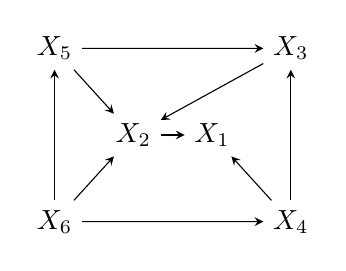
\begin{tikzpicture}[xscale = 1,yscale = 1.1]
        \node (x1) at (1,0) {$X_1$};
        \node (x2) at (0,0) {$X_2$}
          edge [-stealth] (x1);
        \node (x3) at (2,1) {$X_3$}
          edge [-stealth] (x2);
        \node (x4) at (2,-1) {$X_4$}
          edge [-stealth] (x1)
          edge [-stealth] (x3);
        \node (x5) at (-1,1) {$X_5$}
          edge [-stealth] (x2)
          edge [-stealth] (x3);
        \node (x6) at (-1,-1) {$X_6$}
          edge [-stealth] (x2)
          edge [-stealth] (x4)
          edge [-stealth] (x5);
    \end{tikzpicture}
    \caption{An example graph with targets $\mathbf{T}=\{X_1, X_2\}$ on which SNAP($\infty$) performs more \ac{CI} tests than PC.}
    \label{fig:more_tests_example}
\end{figure}

\subsection{Rough approximation of the expected number of possible ancestors}
\label{app:expectedanc}

In practice, the performance of SNAP  depends on the number of possible ancestors of targets in the graph.
We can get an idea of the expected number of \ac{CI} tests by estimating the expected number of possible ancestors.
We could not find an easy solution to this problem in the literature, so we provide a rough approximation for the expected size of the possible ancestors of $\mathbf{T}$ with empirical results that show that it is a substantial overestimation.

Assume $|\mathbf{T}|$ targets are chosen uniformly from all nodes $\mathbf{V}$ without replacement.
Given the topological order of the graph $1..|\mathbf{V}|$, if the highest target in the ordering is at rank $i$, then the rest of the $|\mathbf{T}-1|$ number of targets had to be chosen from nodes at orders $1..i-1$.
Choosing $|\mathbf{T}-1|$ targets from $i-1$ nodes can be done in $\binom{i-1}{|\mathbf{T}|-1}$ many ways.
Then, the probability of the highest target having rank $i$ is given by the number of ways that can be achieved, i.e., $\binom{i-1}{|\mathbf{T}|-1}$, normalised by all the ways one can choose $|\mathbf{T}|$ targets from all $|\mathbf{V}|$ amount of nodes, i.e. $\binom{|\mathbf{V}|}{|\mathbf{T}|}$, resulting in the probability $\binom{i-1}{|\mathbf{T}|-1} / \binom{|\mathbf{V}|}{|\mathbf{T}|}$.
We get the expected rank of the highest ranking target by taking the expectation over all possible highest ranks $i = |\mathbf{T}| .. |\mathbf{V}|$ as follows:
\begin{equation}\label{eq:exp_anc}
    \hat{M} = \frac{1}{ \binom{|\mathbf{V}|}{|\mathbf{T}|} } \sum_{i = |\mathbf{T}|}^{|\mathbf{V}|} i \binom{{i-1}}{|\mathbf{T}|-1}
\end{equation}

We can now overestimate the size of the possible ancestors of $\mathbf{T}$ by simply considering it to be $M$.
As $|\mathbf{T}|$ increases, this upper bound will become tighter, but it is still a loose overestimation.
As shown in Table~\ref{tab:exp_anc}, we empirically find that the number of possible ancestors is much lower than the above estimate.

\begin{table*}[ht]
\begin{tabular}{@{}lrrrrrr@{}}
\toprule
Nodes        & \multicolumn{1}{c}{50} & \multicolumn{1}{c}{100} & \multicolumn{1}{c}{150} & \multicolumn{1}{c}{200} & \multicolumn{1}{c}{250} & \multicolumn{1}{c}{300} \\ \midrule
$\bar{M}$   & $19.64 (\pm 7.16)$     & $23.95 (\pm 10.85)$     & $26.88 (\pm 13.60)$     & $29.49 (\pm 18.66)$     & $28.18 (\pm 15.50)$     & $33.78 (\pm 17.97)$     \\
$\hat{M}$ & $40.8$                 & $80.8$                  & $120.8$                 & $160.8$                 & $200.8$                 & $240.8$                 \\ \bottomrule
\end{tabular}
\caption{Estimates for the expected number of possible ancestors empirically ($\bar{M}$ ) over 100 seeds with various numbers of nodes, $n_{\mathbf{T}}=4, \overline{d} = 3$ and $d_{\max}=10$ in the first row, and by using the Equation~\ref{eq:exp_anc} in the second row ($\hat{M}$).}
\label{tab:exp_anc}
\end{table*}

It is important to note that for any number of possible ancestors of $\mathbf{T}$, SNAP($k$) + PC with $k=0,1$ performs at most as many CI tests as PC, since we do not apply the RFCI rules yet for these $k$. Hence, while such cases can limit the benefits of pruning, low order pruning ($k=0,1$) does not have any downside in terms of CI tests.


\section{EXPERIMENTAL DETAILS}
\label{app:experimental_details}

For our experiments, we used the following libraries: igraph \citep{csardi2006igraph} (GNU GPL version 2 or later), networkx \citep{hagberg2008exploring} (3-Clause BSD License), bnlearn \citep{scutari2010bnlearn} (MIT License), pcalg \citep{kalisch2012pcalg} (GNU GPL version 2 or later), dagitty \citep{textor2016dagitty} (GNU GPL), tetrad \citep{ramsey23pytetrad} (MIT License), causal-learn \citep{zheng2024causal} (MIT License) and RCD \citep{mokhtarian2024recursive} (BSD 2-Clause License).
In particular, we used the \ac{CI} test implementations and some orientation rules from the \texttt{causal-learn} package \citep{zheng2024causal}.
All experiments were performed on AMD Rome CPUs, using 48 CPU cores and 84 GiB of memory.
We let each experiment run for at most 24 hours.
If an experiment did not finish in the given time, we do not report any results for it.

\subsection{Speeding up local algorithms}
\label{sec:local_speed}
For LDECC* and MB-by-MB* we adapt the publicly available code\footnote{GitHub repository of \citet{gupta2023local}: \url{https://github.com/acmi-lab/local-causal-discovery}} of \citet{gupta2023local}.
In particular, we noticed that the running times of these algorithms were much slower than indicated by the number of tests they performed.
We found that this was caused by unnecessary \texttt{deepcopy} operations in their subroutines, thus we removed those.
This means that running times reported here are potentially faster than what one would achieve by using the original codebase.

\subsection{Real-world networks}
\label{app:real_networks}
The MAGIC-NIAB network has 66 nodes, an average degree 3, and is parameterized by linear Gaussian data.
We show the network structure of MAGIC-NIAB in Fig.~\ref{fig:magic-niab}.
The Andes network has 223 nodes, an average degree 3.03, and is parameterized by binary data.
We show the network structure of Andes in Fig.~\ref{fig:andes}.

\begin{figure}
    \centering
    \includegraphics[width=.8\linewidth]{experiments/bnlearn/magic-niab.pdf}
    \caption{The MAGIC-NIAB network.}
    \label{fig:magic-niab}
\end{figure}

\begin{figure}
    \centering
    \includegraphics[width=\linewidth]{experiments/bnlearn/andes.pdf}
    \caption{The Andes network.}
    \label{fig:andes}
\end{figure}

\subsection{Intervention distance} \label{app:metrics}
As one of the main metrics to evaluate the quality of the causal effect estimation, we considered the intervention distance between the estimated causal effect and the ground truth causal effect between pairs of target variables.

We developed this metric in order to be able to estimate the quality of the output even in cases in which the causal effects were not identifiable in the estimated causal graph. This allowed us to compare with all baselines on all the simulated graphs, instead of only focusing on a subset of graphs on which all baselines agreed that the causal effects were identifiable, which could potentially be a very biased set of graphs.

Formally, we then define the intervention distance as follows:
\begin{definition}
\label{def:intervention_distance}
Given targets $\mathbf{T} \subseteq \mathbf{V}$, for $T,T' \in \mathbf{T}$ let $\theta^*_{T, T'}$ be the true causal effect of $T$ on $T'$ and let $\hat{\Theta}_{T, T'}$ be the set of estimated causal effects of $T$ on $T'$ according to the output of an algorithm.
Then the intervention distance is defined as
$$
    \frac{1}{|\mathbf{T}|(|\mathbf{T}|-1) }\sum_{T \in \mathbf{T}} \sum_{T' \in \mathbf{T} \setminus \{T\}} \frac{1}{|\hat{\Theta}_{T, T'}|} \sum_{\hat{\theta} \in \hat{\Theta}_{T, T'}} |\theta^*_{T, T'}-\hat{\theta} |
$$
\end{definition}

\section{COMPLETE EXPERIMENTS}
\label{app:additional_experiments}
This section contains additional results to the ones shown in the main paper, as well as our results for all ablations.
App.~\ref{app:over_nodes} shows additional results on all metrics for graphs with various number of nodes.
App.~\ref{app:identifiable} shows our results for graphs with various number of nodes and with identifiable targets.
We present various ablations in App.~\ref{app:over_targets}, \ref{app:over_degrees} and \ref{app:over_samples} for varying number of targets, expected degree and number of data samples respectively.
App.~\ref{app:snapk} compares SNAP($k$) for $k=0,1,2$.
App.~\ref{app:order} provides a visual explanation on how SNAP variants avoid higher order \ac{CI} tests.
Finally, App.~\ref{app:real-network-results} shows all of our results for the MAGIC-NIAB and the Andes networks.

\subsection{Various number of nodes}
\label{app:over_nodes}
In this section, we consider the same setting presented in the main paper, in Figures~\ref{fig:test_and_time_per_node_unrest_std} and \ref{fig:delta_time_per_node_unrest}, i.e., graphs with various number of nodes, $n_{\mathbf{T}}=4, \overline{d} = 3, d_{\max}=10$ and $n_{\mathbf{D}} = 1000$ data-points.
Fig.~\ref{fig:quality_per_node_unrest_std} shows that intervention distance is not significantly different between most methods.
Fig~\ref{fig:tests_and_time_per_node_unrest} highlights the advantages of different SNAP variants over various settings.
In particular, SNAP($0$) combined with MARVEL or MB-by-MB seems to perform the fewest d-separation tests.
On the other hand, SNAP($\infty$) seems to do best with KCI tests.
On binary data, even though the computation time of FGES trails behind other methods, when combined with SNAP($0$) it becomes the fastest method on this setting.

Figures~\ref{fig:quality_per_node_unrest_std} and \ref{fig:quality_per_node_unrest} show the quality of the estimated structures in terms of \ac{SHD} and intervention distance.
Our results show that even though SNAP variants achieve higher \ac{SHD}, especially when using Fisher-Z tests, their intervention distance is competitive with baselines.
This indicates that structural metrics may not be suitable when the final objective is causal effect estimation.
Additionally, our results for intervention distance in the case of d-separation tests validate that parent adjustment sets are suboptimal for causal effect estimation.

\begin{figure}
    \centering
    \includegraphics[width=.6\linewidth]{experiments/legend_big.pdf}
    % Number of \ac{CI} tests.
    \begin{subfigure}[b]{\linewidth}
        \begin{subfigure}[b]{0.24\linewidth}
            \includegraphics[width=\linewidth]{experiments/per_node/unrestricted/dsep/test_per_node_unrest_dsep.pdf}
            \caption*{d-separation tests}
            \label{fig:test_per_node_unrest_dsep}
        \end{subfigure}
        \begin{subfigure}[b]{0.24\linewidth}
            \includegraphics[width=\linewidth]{experiments/per_node/unrestricted/fshz/test_per_node_unrest_fshz.pdf}
            \caption*{Fisher-Z tests}
            \label{fig:test_per_node_unrest_fshz}
        \end{subfigure}
        \begin{subfigure}[b]{0.24\linewidth}
            \includegraphics[width=\linewidth]{experiments/per_node/unrestricted/kci/test_per_node_unrest_kci.pdf}
            \caption*{KCI tests}
            \label{fig:test_per_node_unrest_kci}
        \end{subfigure}
        \begin{subfigure}[b]{0.24\linewidth}
            \includegraphics[width=\linewidth]{experiments/per_node/unrestricted/chsq/test_per_node_unrest_chsq.pdf}
            \caption*{$\chi^2$ tests}
            \label{fig:test_per_node_unrest_chsq}
        \end{subfigure}
        \caption{Number of \ac{CI} tests.}
        \label{test_per_node_unrest}
    \end{subfigure}
    % Computation time
    \begin{subfigure}[b]{\linewidth}
        \begin{subfigure}[b]{0.25\linewidth}
            \includegraphics[width=\linewidth]{experiments/per_node/unrestricted/dsep/time_per_node_unrest_dsep.pdf}
            \caption*{d-separation tests}
            \label{fig:time_per_node_unrest_dsep}
        \end{subfigure}
        \begin{subfigure}[b]{0.24\linewidth}
            \includegraphics[width=\linewidth]{experiments/per_node/unrestricted/fshz/time_per_node_unrest_fshz.pdf}
            \caption*{Fisher-Z tests}
            \label{fig:time_per_node_unrest_fshz}
        \end{subfigure}
        \begin{subfigure}[b]{0.25\linewidth}
            \includegraphics[width=\linewidth]{experiments/per_node/unrestricted/kci/time_per_node_unrest_kci.pdf}
            \caption*{KCI tests}
            \label{fig:time_per_node_unrest_kci}
        \end{subfigure}
        \begin{subfigure}[b]{0.24\linewidth}
            \includegraphics[width=\linewidth]{experiments/per_node/unrestricted/chsq/time_per_node_unrest_chsq.pdf}
            \caption*{$\chi^2$ tests}
            \label{fig:time_per_node_unrest_chsq}
        \end{subfigure}
        \caption{Computation time.}
        \label{time_per_node_unrest}
    \end{subfigure}
    \caption{Number of \ac{CI} tests and computation time for baseline methods combined with SNAP$(0)$ over number of nodes, with $n_{\mathbf{T}}=4, \overline{d} = 3, d_{\max}=10$ and $n_{\mathbf{D}} = 1000$ data-points.
    }
    \label{fig:tests_and_time_per_node_unrest}
\end{figure}


\begin{figure}
    \centering
    \includegraphics[width=.6\linewidth]{experiments/legend_small.pdf}
    \begin{subfigure}[b]{\linewidth}
        \begin{subfigure}[b]{0.24\linewidth}
            \caption*{d-separation tests}
        \end{subfigure}
        \begin{subfigure}[b]{0.24\linewidth}
            \caption*{Fisher-Z tests}
        \end{subfigure}
        \begin{subfigure}[b]{0.24\linewidth}
            \caption*{KCI tests}
        \end{subfigure}
        \begin{subfigure}[b]{0.24\linewidth}
            \caption*{$\chi^2$ tests}
        \end{subfigure}
    \end{subfigure}
    \begin{subfigure}[b]{\linewidth}
        \begin{subfigure}[b]{0.24\linewidth}
            \includegraphics[width=\linewidth]{experiments/per_node/unrestricted/dsep/int_dist_per_node_unrest_dsep_abs_std.pdf}
        \end{subfigure}
        \begin{subfigure}[b]{0.24\linewidth}
            \includegraphics[width=\linewidth]{experiments/per_node/unrestricted/fshz/int_dist_per_node_unrest_fshz_abs_std.pdf}
        \end{subfigure}
        \begin{subfigure}[b]{0.24\linewidth}
            \includegraphics[width=\linewidth]{experiments/per_node/unrestricted/kci/int_dist_per_node_unrest_kci_abs_std.pdf}
        \end{subfigure}
        \begin{subfigure}[b]{0.24\linewidth}
            \includegraphics[width=\linewidth]{experiments/per_node/unrestricted/chsq/int_dist_per_node_unrest_chsq_abs_std.pdf}
        \end{subfigure}
        \caption{Intervention distance.}
        \label{fig:int_dist_per_node_unrest_std}
    \end{subfigure}
    \begin{subfigure}[b]{\linewidth}
        \begin{subfigure}[b]{0.24\linewidth}
            \includegraphics[width=\linewidth]{experiments/per_node/unrestricted/dsep/shd_per_node_unrest_dsep_std.pdf}
        \end{subfigure}
        \begin{subfigure}[b]{0.24\linewidth}
            \includegraphics[width=\linewidth]{experiments/per_node/unrestricted/fshz/shd_per_node_unrest_fshz_std.pdf}
        \end{subfigure}
        \begin{subfigure}[b]{0.24\linewidth}
            \includegraphics[width=\linewidth]{experiments/per_node/unrestricted/kci/shd_per_node_unrest_kci_std.pdf}
        \end{subfigure}
        \begin{subfigure}[b]{0.24\linewidth}
            \includegraphics[width=\linewidth]{experiments/per_node/unrestricted/chsq/shd_per_node_unrest_chsq_std.pdf}
        \end{subfigure}
        \caption{\Acf{SHD}.}
        \label{fig:shd_per_node_unrest_std}
    \end{subfigure}
    \caption{Quality of estimation over number of nodes, with $n_{\mathbf{T}}=4, \overline{d} = 3, d_{\max}=10$ and $n_{\mathbf{D}} = 1000$ data-points. We compute the intervention distance in the d-separation tests case using random linear Gaussian data according to the discovered structure.}
    \label{fig:quality_per_node_unrest_std}
\end{figure}

\begin{figure}
    \centering
    \includegraphics[width=.6\linewidth]{experiments/legend_big.pdf}
    % Intervention distance.
    \begin{subfigure}[b]{\linewidth}
        \begin{subfigure}[b]{0.24\linewidth}
            \includegraphics[width=\linewidth]{experiments/per_node/unrestricted/dsep/int_dist_per_node_unrest_dsep_abs.pdf}
            \caption*{d-separation tests}
            \label{fig:int_dist_per_node_unrest_dsep_abs}
        \end{subfigure}
        \begin{subfigure}[b]{0.24\linewidth}
            \includegraphics[width=\linewidth]{experiments/per_node/unrestricted/fshz/int_dist_per_node_unrest_fshz_abs.pdf}
            \caption*{Fisher-Z tests}
            \label{fig:int_dist_per_node_unrest_fshz_abs}
        \end{subfigure}
        \begin{subfigure}[b]{0.24\linewidth}
            \includegraphics[width=\linewidth]{experiments/per_node/unrestricted/kci/int_dist_per_node_unrest_kci_abs.pdf}
            \caption*{KCI tests}
            \label{fig:int_dist_per_node_unrest_kci_abs}
        \end{subfigure}
        \begin{subfigure}[b]{0.24\linewidth}
            \includegraphics[width=\linewidth]{experiments/per_node/unrestricted/chsq/int_dist_per_node_unrest_chsq_abs.pdf}
            \caption*{$\chi^2$ tests}
            \label{fig:int_dist_per_node_unrest_chsq_abs}
        \end{subfigure}
        \caption{Intervention distance.}
        \label{fig:int_dist_per_node_unrest}
    \end{subfigure}
    % SHD
    \begin{subfigure}[b]{\linewidth}
        \begin{subfigure}[b]{0.24\linewidth}
            \includegraphics[width=\linewidth]{experiments/per_node/unrestricted/dsep/shd_per_node_unrest_dsep.pdf}
            \caption*{d-separation tests}
            \label{fig:shd_per_node_unrest_dsep}
        \end{subfigure}
        \begin{subfigure}[b]{0.24\linewidth}
            \includegraphics[width=\linewidth]{experiments/per_node/unrestricted/fshz/shd_per_node_unrest_fshz.pdf}
            \caption*{Fisher-Z tests}
            \label{fig:shd_per_node_unrest_fshz}
        \end{subfigure}
        \begin{subfigure}[b]{0.24\linewidth}
            \includegraphics[width=\linewidth]{experiments/per_node/unrestricted/kci/shd_per_node_unrest_kci.pdf}
            \caption*{KCI tests}
            \label{fig:shd_per_node_unrest_kci}
        \end{subfigure}
        \begin{subfigure}[b]{0.24\linewidth}
            \includegraphics[width=\linewidth]{experiments/per_node/unrestricted/chsq/shd_per_node_unrest_chsq.pdf}
            \caption*{$\chi^2$ tests}
            \label{fig:shd_per_node_unrest_chsq}
        \end{subfigure}
        \caption{\Acf{SHD}.}
        \label{fig:shd_per_node_unrest}
    \end{subfigure}
    \caption{Quality of estimation over number of nodes for baseline methods combined with SNAP$(0)$, with $n_{\mathbf{T}}=4, \overline{d} = 3, d_{\max}=10$ and $n_{\mathbf{D}} = 1000$ data-points. We compute the intervention distance in the d-separation tests case using random linear Gaussian data according to the discovered structure.}
    \label{fig:quality_per_node_unrest}
\end{figure}


\subsection{Identifiable targets}
\label{app:identifiable}
In this section, we sample target sets for experiment that are \emph{identifiable}.
We consider a set of targets identifiable if the causal effect is identifiable from the true CPDAG between each pair of targets.
To ensure that these identifiable causal effects are not mostly zero, when sampling identifiable targets, we also require that they are the ancestor or the descendant of at least one other target.
This makes intervention distance more meaningful, as the true CPDAG should achieve a near zero distance, while incorrect and overly sparse \acp{CPDAG} should achieve higher distances.
Furthermore, it allows us to measure the \acf{AID}.

Figures~\ref{fig:appendix_per_node_ident_std} and \ref{fig:appendix_per_node_ident} shows that enforcing targets to be identifiable does not have a significant impact on the results.
\Cref{fig:aid_per_node_ident_std,fig:aid_per_node_ident} show results for \acf{AID}, where SNAP variants are comparable to most methods.
In particular, SNAP$(0)$ improves MARVEL on linear Gaussian data with Fisher-Z tests.
SNAP variants seem to struggle the most on binary data in terms of adjustment identification distance.

\begin{figure}
    \centering
    \includegraphics[width=.6\linewidth]{experiments/legend_small.pdf}
    % Number of CI tests
    \begin{subfigure}[b]{\linewidth}
        \begin{subfigure}[b]{0.24\linewidth}
            \includegraphics[width=\linewidth]{experiments/per_node/identifiable/dsep/test_per_node_ident_dsep_std.pdf}
            \caption*{d-separation tests}
            \label{fig:test_per_node_ident_dsep_std}
        \end{subfigure}
        \begin{subfigure}[b]{0.24\linewidth}
            \includegraphics[width=\linewidth]{experiments/per_node/identifiable/fshz/test_per_node_ident_fshz_std.pdf}
            \caption*{Fisher-Z tests}
            \label{fig:test_per_node_ident_fshz_std}
        \end{subfigure}
        \begin{subfigure}[b]{0.24\linewidth}
            \includegraphics[width=\linewidth]{experiments/per_node/identifiable/kci/test_per_node_ident_kci_std.pdf}
            \caption*{KCI tests}
            \label{fig:test_per_node_ident_kci_std}
        \end{subfigure}
        \begin{subfigure}[b]{0.24\linewidth}
            \includegraphics[width=\linewidth]{experiments/per_node/identifiable/chsq/test_per_node_ident_chsq_std.pdf}
            \caption*{$\chi^2$ tests}
            \label{fig:test_per_node_ident_chsq_std}
        \end{subfigure}
        \caption{Number of \ac{CI} tests.}
        \label{fig:test_per_node_ident_std}
    \end{subfigure}
    % Computation time
    \begin{subfigure}[b]{\linewidth}
        \begin{subfigure}[b]{0.24\linewidth}
            \includegraphics[width=\linewidth]{experiments/per_node/identifiable/dsep/time_per_node_ident_dsep_std.pdf}
            \caption*{d-separation tests}
            \label{fig:time_per_node_ident_dsep_std}
        \end{subfigure}
        \begin{subfigure}[b]{0.24\linewidth}
            \includegraphics[width=\linewidth]{experiments/per_node/identifiable/fshz/time_per_node_ident_fshz_std.pdf}
            \caption*{Fisher-Z tests}
            \label{fig:time_per_node_ident_fshz_std}
        \end{subfigure}
        \begin{subfigure}[b]{0.24\linewidth}
            \includegraphics[width=\linewidth]{experiments/per_node/identifiable/kci/time_per_node_ident_kci_std.pdf}
            \caption*{KCI tests}
            \label{fig:time_per_node_ident_kci_std}
        \end{subfigure}
        \begin{subfigure}[b]{0.24\linewidth}
            \includegraphics[width=\linewidth]{experiments/per_node/identifiable/chsq/time_per_node_ident_chsq_std.pdf}
            \caption*{$\chi^2$ tests}
            \label{fig:time_per_node_ident_chsq_std}
        \end{subfigure}
        \caption{Computation time.}
        \label{fig:time_per_node_ident_std}
    \end{subfigure}
    
    % Intervention distance
    \begin{subfigure}[b]{\linewidth}
        \begin{subfigure}[b]{0.24\linewidth}
            \includegraphics[width=\linewidth]{experiments/per_node/identifiable/dsep/int_dist_per_node_ident_dsep_abs_std.pdf}
            \caption*{d-separation tests}
            \label{fig:int_dist_per_node_ident_dsep_abs_std}
        \end{subfigure}
        \begin{subfigure}[b]{0.24\linewidth}
            \includegraphics[width=\linewidth]{experiments/per_node/identifiable/fshz/int_dist_per_node_ident_fshz_abs_std.pdf}
            \caption*{Fisher-Z tests}
            \label{fig:int_dist_per_node_ident_fshz_abs_std}
        \end{subfigure}
        \begin{subfigure}[b]{0.24\linewidth}
            \includegraphics[width=\linewidth]{experiments/per_node/identifiable/kci/int_dist_per_node_ident_kci_abs_std.pdf}
            \caption*{KCI tests}
            \label{fig:int_dist_per_node_ident_kci_abs_std}
        \end{subfigure}
        \begin{subfigure}[b]{0.24\linewidth}
            \includegraphics[width=\linewidth]{experiments/per_node/identifiable/chsq/int_dist_per_node_ident_chsq_abs_std.pdf}
            \caption*{$\chi^2$ tests}
            \label{fig:int_dist_per_node_ident_chsq_abs_std}
        \end{subfigure}
        \caption{Intervention distance.}
        \label{fig:int_dist_per_node_ident_std}
    \end{subfigure}
    % SHD
    \begin{subfigure}[b]{\linewidth}
        \begin{subfigure}[b]{0.24\linewidth}
            \includegraphics[width=\linewidth]{experiments/per_node/identifiable/dsep/shd_per_node_ident_dsep_std.pdf}
            \caption*{d-separation tests}
            \label{fig:shd_per_node_ident_dsep_std}
        \end{subfigure}
        \begin{subfigure}[b]{0.24\linewidth}
            \includegraphics[width=\linewidth]{experiments/per_node/identifiable/fshz/shd_per_node_ident_fshz_std.pdf}
            \caption*{Fisher-Z tests}
            \label{fig:shd_per_node_ident_fshz_std}
        \end{subfigure}
        \begin{subfigure}[b]{0.24\linewidth}
            \includegraphics[width=\linewidth]{experiments/per_node/identifiable/kci/shd_per_node_ident_kci_std.pdf}
            \caption*{KCI tests}
            \label{fig:shd_per_node_ident_kci_std}
        \end{subfigure}
        \begin{subfigure}[b]{0.24\linewidth}
            \includegraphics[width=\linewidth]{experiments/per_node/identifiable/chsq/shd_per_node_ident_chsq_std.pdf}
            \caption*{$\chi^2$ tests}
            \label{fig:shd_per_node_ident_chsq_std}
        \end{subfigure}
        \caption{\Acf{SHD}.}
        \label{fig:shd_per_node_ident_std}
    \end{subfigure}
    \caption{Additional results over number of nodes for identifiable targets, with $n_{\mathbf{T}}=4, \overline{d} = 3, d_{\max}=10$ and $n_{\mathbf{D}} = 1000$ data-points. The shadow area denotes the range of the standard deviation. We compute the intervention distance in the d-separation tests case using random linear Gaussian data according to the discovered structure.}
    \label{fig:appendix_per_node_ident_std}
\end{figure}

\begin{figure}
    \centering
    \includegraphics[width=.6\linewidth]{experiments/legend_big.pdf}
    % Number of tests
    \begin{subfigure}[b]{\linewidth}
        \begin{subfigure}[b]{0.24\linewidth}
            \includegraphics[width=\linewidth]{experiments/per_node/identifiable/dsep/test_per_node_ident_dsep.pdf}
            \caption*{d-separation tests}
            \label{fig:test_per_node_ident_dsep}
        \end{subfigure}
        \begin{subfigure}[b]{0.24\linewidth}
            \includegraphics[width=\linewidth]{experiments/per_node/identifiable/fshz/test_per_node_ident_fshz.pdf}
            \caption*{Fisher-Z tests}
            \label{fig:test_per_node_ident_fshz}
        \end{subfigure}
        \begin{subfigure}[b]{0.24\linewidth}
            \includegraphics[width=\linewidth]{experiments/per_node/identifiable/kci/test_per_node_ident_kci.pdf}
            \caption*{KCI tests}
            \label{fig:test_per_node_ident_kci}
        \end{subfigure}
        \begin{subfigure}[b]{0.24\linewidth}
            \includegraphics[width=\linewidth]{experiments/per_node/identifiable/chsq/test_per_node_ident_chsq.pdf}
            \caption*{$\chi^2$ tests}
            \label{fig:test_per_node_ident_chsq}
        \end{subfigure}
        \caption{Number of \ac{CI} tests.}
        \label{fig:test_per_node_ident}
    \end{subfigure}
    % Computation time
    \begin{subfigure}[b]{\linewidth}
        \begin{subfigure}[b]{0.24\linewidth}
            \includegraphics[width=\linewidth]{experiments/per_node/identifiable/dsep/time_per_node_ident_dsep.pdf}
            \caption*{d-separation tests}
            \label{fig:time_per_node_ident_dsep}
        \end{subfigure}
        \begin{subfigure}[b]{0.24\linewidth}
            \includegraphics[width=\linewidth]{experiments/per_node/identifiable/fshz/time_per_node_ident_fshz.pdf}
            \caption*{Fisher-Z tests}
            \label{fig:time_per_node_ident_fshz}
        \end{subfigure}
        \begin{subfigure}[b]{0.24\linewidth}
            \includegraphics[width=\linewidth]{experiments/per_node/identifiable/kci/time_per_node_ident_kci.pdf}
            \caption*{KCI tests}
            \label{fig:time_per_node_ident_kci}
        \end{subfigure}
        \begin{subfigure}[b]{0.24\linewidth}
            \includegraphics[width=\linewidth]{experiments/per_node/identifiable/chsq/time_per_node_ident_chsq.pdf}
            \caption*{$\chi^2$ tests}
            \label{fig:time_per_node_ident_chsq}
        \end{subfigure}
        \caption{Computation time.}
        \label{fig:time_per_node_ident}
    \end{subfigure}
    % Intervention distance
    \begin{subfigure}[b]{\linewidth}
        \begin{subfigure}[b]{0.24\linewidth}
            \includegraphics[width=\linewidth]{experiments/per_node/identifiable/dsep/int_dist_per_node_ident_dsep_abs.pdf}
            \caption*{d-separation tests}
            \label{fig:int_dist_per_node_ident_dsep_abs}
        \end{subfigure}
        \begin{subfigure}[b]{0.24\linewidth}
            \includegraphics[width=\linewidth]{experiments/per_node/identifiable/fshz/int_dist_per_node_ident_fshz_abs.pdf}
            \caption*{Fisher-Z tests}
            \label{fig:int_dist_per_node_ident_fshz_abs}
        \end{subfigure}
        \begin{subfigure}[b]{0.24\linewidth}
            \includegraphics[width=\linewidth]{experiments/per_node/identifiable/kci/int_dist_per_node_ident_kci_abs.pdf}
            \caption*{KCI tests}
            \label{fig:int_dist_per_node_ident_kci_abs}
        \end{subfigure}
        \begin{subfigure}[b]{0.24\linewidth}
            \includegraphics[width=\linewidth]{experiments/per_node/identifiable/chsq/int_dist_per_node_ident_chsq_abs.pdf}
            \caption*{$\chi^2$ tests}
            \label{fig:int_dist_per_node_ident_chsq_abs}
        \end{subfigure}
        \caption{Intervention distance.}
        \label{fig:int_dist_per_node_ident}
    \end{subfigure}
    % SHD
    \begin{subfigure}[b]{\linewidth}
        \begin{subfigure}[b]{0.24\linewidth}
            \includegraphics[width=\linewidth]{experiments/per_node/identifiable/dsep/shd_per_node_ident_dsep.pdf}
            \caption*{d-separation tests}
            \label{fig:shd_per_node_ident_dsep}
        \end{subfigure}
        \begin{subfigure}[b]{0.24\linewidth}
            \includegraphics[width=\linewidth]{experiments/per_node/identifiable/fshz/shd_per_node_ident_fshz.pdf}
            \caption*{Fisher-Z tests}
            \label{fig:shd_per_node_ident_fshz}
        \end{subfigure}
        \begin{subfigure}[b]{0.24\linewidth}
            \includegraphics[width=\linewidth]{experiments/per_node/identifiable/kci/shd_per_node_ident_kci.pdf}
            \caption*{KCI tests}
            \label{fig:shd_per_node_ident_kci}
        \end{subfigure}
        \begin{subfigure}[b]{0.24\linewidth}
            \includegraphics[width=\linewidth]{experiments/per_node/identifiable/chsq/shd_per_node_ident_chsq.pdf}
            \caption*{$\chi^2$ tests}
            \label{fig:shd_per_node_ident_chsq}
        \end{subfigure}
        \caption{\Acf{SHD}.}
        \label{fig:shd_per_node_ident}
    \end{subfigure}
    \caption{Additional results over number of nodes for identifiable targets, with $n_{\mathbf{T}}=4, \overline{d} = 3, d_{\max}=10$ and $n_{\mathbf{D}} = 1000$ data-points. We also show baseline methods combined with SNAP$(0)$. We compute the intervention distance in the d-separation tests case using random linear Gaussian data according to the discovered structure.}
    \label{fig:appendix_per_node_ident}
\end{figure}

\begin{figure}
    \centering
    \includegraphics[width=.6\linewidth]{experiments/legend_small.pdf}
    % Parent-AID
    \begin{subfigure}[b]{\linewidth}
        \begin{subfigure}[b]{0.24\linewidth}
            \includegraphics[width=\linewidth]{experiments/per_node/identifiable/dsep/parent_aid_per_node_ident_dsep_std.pdf}
            \caption*{d-separation tests}
            \label{fig:parent_aid_per_node_ident_dsep_std}
        \end{subfigure}
        \begin{subfigure}[b]{0.24\linewidth}
            \includegraphics[width=\linewidth]{experiments/per_node/identifiable/fshz/parent_aid_per_node_ident_fshz_std.pdf}
            \caption*{Fisher-Z tests}
            \label{fig:parent_aid_per_node_ident_fshz_std}
        \end{subfigure}
        \begin{subfigure}[b]{0.24\linewidth}
            \includegraphics[width=\linewidth]{experiments/per_node/identifiable/kci/parent_aid_per_node_ident_kci_std.pdf}
            \caption*{KCI tests}
            \label{fig:parent_aid_per_node_ident_kci_std}
        \end{subfigure}
        \begin{subfigure}[b]{0.24\linewidth}
            \includegraphics[width=\linewidth]{experiments/per_node/identifiable/chsq/parent_aid_per_node_ident_chsq_std.pdf}
            \caption*{$\chi^2$ tests}
            \label{fig:parent_aid_per_node_ident_chsq_std}
        \end{subfigure}
        \caption{Parent-AID.}
        \label{fig:parent_aid_per_node_ident_std}
    \end{subfigure}
    % Ancestor-AID
    \begin{subfigure}[b]{\linewidth}
        \begin{subfigure}[b]{0.24\linewidth}
            \includegraphics[width=\linewidth]{experiments/per_node/identifiable/dsep/ancestor_aid_per_node_ident_dsep_std.pdf}
            \caption*{d-separation tests}
            \label{fig:ancestor_aid_per_node_ident_dsep_std}
        \end{subfigure}
        \begin{subfigure}[b]{0.24\linewidth}
            \includegraphics[width=\linewidth]{experiments/per_node/identifiable/fshz/ancestor_aid_per_node_ident_fshz_std.pdf}
            \caption*{Fisher-Z tests}
            \label{fig:ancestor_aid_per_node_ident_fshz_std}
        \end{subfigure}
        \begin{subfigure}[b]{0.24\linewidth}
            \includegraphics[width=\linewidth]{experiments/per_node/identifiable/kci/ancestor_aid_per_node_ident_kci_std.pdf}
            \caption*{KCI tests}
            \label{fig:ancestor_aid_per_node_ident_kci_std}
        \end{subfigure}
        \begin{subfigure}[b]{0.24\linewidth}
            \includegraphics[width=\linewidth]{experiments/per_node/identifiable/chsq/ancestor_aid_per_node_ident_chsq_std.pdf}
            \caption*{$\chi^2$ tests}
            \label{fig:ancestor_aid_per_node_ident_chsq_std}
        \end{subfigure}
        \caption{Ancestor-AID.}
        \label{fig:ancestor_aid_per_node_ident_std}
    \end{subfigure}
    % Oset-AID
    \begin{subfigure}[b]{\linewidth}
        \begin{subfigure}[b]{0.24\linewidth}
            \includegraphics[width=\linewidth]{experiments/per_node/identifiable/dsep/oset_aid_per_node_ident_dsep_std.pdf}
            \caption*{d-separation tests}
            \label{fig:oset_aid_per_node_ident_dsep_std}
        \end{subfigure}
        \begin{subfigure}[b]{0.24\linewidth}
            \includegraphics[width=\linewidth]{experiments/per_node/identifiable/fshz/oset_aid_per_node_ident_fshz_std.pdf}
            \caption*{Fisher-Z tests}
            \label{fig:oset_aid_per_node_ident_fshz_std}
        \end{subfigure}
        \begin{subfigure}[b]{0.24\linewidth}
            \includegraphics[width=\linewidth]{experiments/per_node/identifiable/kci/oset_aid_per_node_ident_kci_std.pdf}
            \caption*{KCI tests}
            \label{fig:oset_aid_per_node_ident_kci_std}
        \end{subfigure}
        \begin{subfigure}[b]{0.24\linewidth}
            \includegraphics[width=\linewidth]{experiments/per_node/identifiable/chsq/oset_aid_per_node_ident_chsq_std.pdf}
            \caption*{$\chi^2$ tests}
            \label{fig:oset_aid_per_node_ident_chsq_std}
        \end{subfigure}
        \caption{Oset-AID.}
        \label{fig:oset_aid_per_node_ident_std}
    \end{subfigure}
    \caption{Adjustment identification distance over number of nodes for identifiable targets, with $n_{\mathbf{T}}=4, \overline{d} = 3, d_{\max}=10$ and $n_{\mathbf{D}} = 1000$ data-points. The shadow area denotes the range of the standard deviation.}
    \label{fig:aid_per_node_ident_std}
\end{figure}

\begin{figure}
    \centering
    \includegraphics[width=.6\linewidth]{experiments/legend_big.pdf}
    % Parent-AID
    \begin{subfigure}[b]{\linewidth}
        \begin{subfigure}[b]{0.24\linewidth}
            \includegraphics[width=\linewidth]{experiments/per_node/identifiable/dsep/parent_aid_per_node_ident_dsep.pdf}
            \caption*{d-separation tests}
            \label{fig:parent_aid_per_node_ident_dsep}
        \end{subfigure}
        \begin{subfigure}[b]{0.24\linewidth}
            \includegraphics[width=\linewidth]{experiments/per_node/identifiable/fshz/parent_aid_per_node_ident_fshz.pdf}
            \caption*{Fisher-Z tests}
            \label{fig:parent_aid_per_node_ident_fshz}
        \end{subfigure}
        \begin{subfigure}[b]{0.24\linewidth}
            \includegraphics[width=\linewidth]{experiments/per_node/identifiable/kci/parent_aid_per_node_ident_kci.pdf}
            \caption*{KCI tests}
            \label{fig:parent_aid_per_node_ident_kci}
        \end{subfigure}
        \begin{subfigure}[b]{0.24\linewidth}
            \includegraphics[width=\linewidth]{experiments/per_node/identifiable/chsq/parent_aid_per_node_ident_chsq.pdf}
            \caption*{$\chi^2$ tests}
            \label{fig:parent_aid_per_node_ident_chsq}
        \end{subfigure}
        \caption{Parent-AID.}
        \label{fig:parent_aid_per_node_ident}
    \end{subfigure}
    % Ancestor-AID
    \begin{subfigure}[b]{\linewidth}
        \begin{subfigure}[b]{0.24\linewidth}
            \includegraphics[width=\linewidth]{experiments/per_node/identifiable/dsep/ancestor_aid_per_node_ident_dsep.pdf}
            \caption*{d-separation tests}
            \label{fig:ancestor_aid_per_node_ident_dsep}
        \end{subfigure}
        \begin{subfigure}[b]{0.24\linewidth}
            \includegraphics[width=\linewidth]{experiments/per_node/identifiable/fshz/ancestor_aid_per_node_ident_fshz.pdf}
            \caption*{Fisher-Z tests}
            \label{fig:ancestor_aid_per_node_ident_fshz}
        \end{subfigure}
        \begin{subfigure}[b]{0.24\linewidth}
            \includegraphics[width=\linewidth]{experiments/per_node/identifiable/kci/ancestor_aid_per_node_ident_kci.pdf}
            \caption*{KCI tests}
            \label{fig:ancestor_aid_per_node_ident_kci}
        \end{subfigure}
        \begin{subfigure}[b]{0.24\linewidth}
            \includegraphics[width=\linewidth]{experiments/per_node/identifiable/chsq/ancestor_aid_per_node_ident_chsq.pdf}
            \caption*{$\chi^2$ tests}
            \label{fig:ancestor_aid_per_node_ident_chsq}
        \end{subfigure}
        \caption{Ancestor-AID.}
        \label{fig:ancestor_aid_per_node_ident}
    \end{subfigure}
    % Oset-AID
    \begin{subfigure}[b]{\linewidth}
        \begin{subfigure}[b]{0.24\linewidth}
            \includegraphics[width=\linewidth]{experiments/per_node/identifiable/dsep/oset_aid_per_node_ident_dsep.pdf}
            \caption*{d-separation tests}
            \label{fig:oset_aid_per_node_ident_dsep}
        \end{subfigure}
        \begin{subfigure}[b]{0.24\linewidth}
            \includegraphics[width=\linewidth]{experiments/per_node/identifiable/fshz/oset_aid_per_node_ident_fshz.pdf}
            \caption*{Fisher-Z tests}
            \label{fig:oset_aid_per_node_ident_fshz}
        \end{subfigure}
        \begin{subfigure}[b]{0.24\linewidth}
            \includegraphics[width=\linewidth]{experiments/per_node/identifiable/kci/oset_aid_per_node_ident_kci.pdf}
            \caption*{KCI tests}
            \label{fig:oset_aid_per_node_ident_kci}
        \end{subfigure}
        \begin{subfigure}[b]{0.24\linewidth}
            \includegraphics[width=\linewidth]{experiments/per_node/identifiable/chsq/oset_aid_per_node_ident_chsq.pdf}
            \caption*{$\chi^2$ tests}
            \label{fig:oset_aid_per_node_ident_chsq}
        \end{subfigure}
        \caption{Oset-AID.}
        \label{fig:oset_aid_per_node_ident}
    \end{subfigure}
    \caption{Adjustment identification distance over number of nodes for identifiable targets, with $n_{\mathbf{T}}=4, \overline{d} = 3, d_{\max}=10$ and $n_{\mathbf{D}} = 1000$ data-points. We also show baseline methods combined with SNAP$(0)$.}
    \label{fig:aid_per_node_ident}
\end{figure}

\subsection{Various numbers of targets}
\label{app:over_targets}

\Cref{fig:computation_per_target_unrest_std,fig:quality_per_target_unrest_std,fig:computation_per_target_unrest,fig:quality_per_target_unrest} and \Cref{fig:computation_per_target_ident_std,fig:quality_per_target_ident_std,fig:computation_per_target_ident,fig:quality_per_target_ident} show results for varying number of random and identifiable targets respectively, with all other parameters fixed.
In terms of \ac{CI} tests and computation time, SNAP is much more robust against different number of targets than local methods, while maintaining a comparable intervention distance.
Furthermore, SHD is only worse compared to other methods when using Fisher-Z tests on linear Gaussian data.

\begin{figure}
    \centering
    \includegraphics[width=.6\linewidth]{experiments/legend_big.pdf}
    % Number of tests
    \begin{subfigure}[b]{\linewidth}
        \centering
        \begin{subfigure}[b]{0.24\linewidth}
            \includegraphics[width=\linewidth]{experiments/per_target/unrestricted/dsep/test_per_target_unrest_dsep_std.pdf}
            \caption*{d-separation tests}
            \label{fig:test_per_target_unrest_dsep_std}
        \end{subfigure}
        \begin{subfigure}[b]{0.24\linewidth}
            \includegraphics[width=\linewidth]{experiments/per_target/unrestricted/fshz/test_per_target_unrest_fshz_std.pdf}
            \caption*{Fisher-Z tests}
            \label{fig:test_per_target_unrest_fshz_std}
        \end{subfigure}
        \begin{subfigure}[b]{0.24\linewidth}
            \includegraphics[width=\linewidth]{experiments/per_target/unrestricted/kci/test_per_target_unrest_kci_std.pdf}
            \caption*{KCI tests}
            \label{fig:test_per_target_unrest_kci_std}
        \end{subfigure}
        \begin{subfigure}[b]{0.24\linewidth}
            \includegraphics[width=\linewidth]{experiments/per_target/unrestricted/chsq/test_per_target_unrest_chsq_std.pdf}
            \caption*{$\chi^2$ tests}
            \label{fig:test_per_target_unrest_chsq_std}
        \end{subfigure}
        \caption{Number of \ac{CI} tests.}
        \label{fig:test_per_target_unrest_std}
    \end{subfigure}
    % Computation time
    \begin{subfigure}[b]{\linewidth}
        \centering
        \begin{subfigure}[b]{0.24\linewidth}
            \includegraphics[width=\linewidth]{experiments/per_target/unrestricted/dsep/time_per_target_unrest_dsep_std.pdf}
            \caption*{d-separation tests}
            \label{fig:time_per_target_unrest_dsep_std}
        \end{subfigure}
        \begin{subfigure}[b]{0.24\linewidth}
            \includegraphics[width=\linewidth]{experiments/per_target/unrestricted/fshz/time_per_target_unrest_fshz_std.pdf}
            \caption*{Fisher-Z tests}
            \label{fig:time_per_target_unrest_fshz_std}
        \end{subfigure}
        \begin{subfigure}[b]{0.24\linewidth}
            \includegraphics[width=\linewidth]{experiments/per_target/unrestricted/kci/time_per_target_unrest_kci_std.pdf}
            \caption*{KCI tests}
            \label{fig:time_per_target_unrest_kci_std}
        \end{subfigure}
        \begin{subfigure}[b]{0.24\linewidth}
            \includegraphics[width=\linewidth]{experiments/per_target/unrestricted/chsq/time_per_target_unrest_chsq_std.pdf}
            \caption*{$\chi^2$ tests}
            \label{fig:time_per_target_unrest_chsq_std}
        \end{subfigure}
        \caption{Computation time.}
        \label{fig:time_per_target_unrest_std}
    \end{subfigure}
    \caption{Number of \ac{CI} tests and computation time over number of targets, with $n_{\mathbf{V}}=10$ for KCI tests and $n_{\mathbf{V}}=200$ otherwise, $\overline{d} = 3, d_{\max}=10$ and $n_{\mathbf{D}} = 1000$ data-points. The shadow area denotes the range of the standard deviation. We plot values on a $\log$ scale.}
    \label{fig:computation_per_target_unrest_std}
\end{figure}

\begin{figure}
    \centering
    \includegraphics[width=.6\linewidth]{experiments/legend_big.pdf}
    % Intervention distance
    \begin{subfigure}[b]{\linewidth}
        \centering
        \begin{subfigure}[b]{0.24\linewidth}
            \includegraphics[width=\linewidth]{experiments/per_target/unrestricted/dsep/int_dist_per_target_unrest_dsep_abs_std.pdf}
            \caption*{d-separation tests}
            \label{fig:int_dist_per_target_unrest_dsep_abs_std}
        \end{subfigure}
        \begin{subfigure}[b]{0.24\linewidth}
            \includegraphics[width=\linewidth]{experiments/per_target/unrestricted/fshz/int_dist_per_target_unrest_fshz_abs_std.pdf}
            \caption*{Fisher-Z tests}
            \label{fig:int_dist_per_target_unrest_fshz_abs_std}
        \end{subfigure}
        \begin{subfigure}[b]{0.24\linewidth}
            \includegraphics[width=\linewidth]{experiments/per_target/unrestricted/kci/int_dist_per_target_unrest_kci_abs_std.pdf}
            \caption*{KCI tests}
            \label{fig:int_dist_per_target_unrest_kci_abs_std}
        \end{subfigure}
        \begin{subfigure}[b]{0.24\linewidth}
            \includegraphics[width=\linewidth]{experiments/per_target/unrestricted/chsq/int_dist_per_target_unrest_chsq_abs_std.pdf}
            \caption*{$\chi^2$ tests}
            \label{fig:int_dist_per_target_unrest_chsq_abs_std}
        \end{subfigure}
        \caption{Intervention distance}
        \label{fig:int_dist_per_target_unrest_abs_std}
    \end{subfigure}
    % SHD
    \begin{subfigure}[b]{\linewidth}
        \centering
        \begin{subfigure}[b]{0.24\linewidth}
            \includegraphics[width=\linewidth]{experiments/per_target/unrestricted/dsep/shd_per_target_unrest_dsep_std.pdf}
            \caption*{d-separation tests}
            \label{fig:shd_per_target_unrest_dsep_std}
        \end{subfigure}
        \begin{subfigure}[b]{0.24\linewidth}
            \includegraphics[width=\linewidth]{experiments/per_target/unrestricted/fshz/shd_per_target_unrest_fshz_std.pdf}
            \caption*{Fisher-Z tests}
            \label{fig:shd_per_target_unrest_fshz_std}
        \end{subfigure}
        \begin{subfigure}[b]{0.24\linewidth}
            \includegraphics[width=\linewidth]{experiments/per_target/unrestricted/kci/shd_per_target_unrest_kci_std.pdf}
            \caption*{KCI tests}
            \label{fig:shd_per_target_unrest_kci_std}
        \end{subfigure}
        \begin{subfigure}[b]{0.24\linewidth}
            \includegraphics[width=\linewidth]{experiments/per_target/unrestricted/chsq/shd_per_target_unrest_chsq_std.pdf}
            \caption*{$\chi^2$ tests}
            \label{fig:shd_per_target_unrest_chsq_std}
        \end{subfigure}
        \caption{\Acl{SHD}}
        \label{fig:shd_per_target_unrest_std}
    \end{subfigure}
    \caption{Estimation quality over number of targets, with $n_{\mathbf{V}}=10$ for KCI tests and $n_{\mathbf{V}}=200$ otherwise, $\overline{d} = 3, d_{\max}=10$ and $n_{\mathbf{D}} = 1000$ data-points. The shadow area denotes the range of the standard deviation.}
    \label{fig:quality_per_target_unrest_std}
\end{figure}

\begin{figure}
    \centering
    \includegraphics[width=.6\linewidth]{experiments/legend_big.pdf}
    % Number of tests
    \begin{subfigure}[b]{\linewidth}
        \centering
        \begin{subfigure}[b]{0.24\linewidth}
            \includegraphics[width=\linewidth]{experiments/per_target/unrestricted/dsep/test_per_target_unrest_dsep.pdf}
            \caption*{d-separation tests}
            \label{fig:test_per_target_unrest_dsep}
        \end{subfigure}
        \begin{subfigure}[b]{0.24\linewidth}
            \includegraphics[width=\linewidth]{experiments/per_target/unrestricted/fshz/test_per_target_unrest_fshz.pdf}
            \caption*{Fisher-Z tests}
            \label{fig:test_per_target_unrest_fshz}
        \end{subfigure}
        \begin{subfigure}[b]{0.24\linewidth}
            \includegraphics[width=\linewidth]{experiments/per_target/unrestricted/kci/test_per_target_unrest_kci.pdf}
            \caption*{KCI tests}
            \label{fig:test_per_target_unrest_kci}
        \end{subfigure}
        \begin{subfigure}[b]{0.24\linewidth}
            \includegraphics[width=\linewidth]{experiments/per_target/unrestricted/chsq/test_per_target_unrest_chsq.pdf}
            \caption*{$\chi^2$ tests}
            \label{fig:test_per_target_unrest_chsq}
        \end{subfigure}
        \caption{Number of \ac{CI} tests.}
        \label{fig:test_per_target_unrest_no}
    \end{subfigure}
    % Computation time
    \begin{subfigure}[b]{\linewidth}
        \centering
        \begin{subfigure}[b]{0.24\linewidth}
            \includegraphics[width=\linewidth]{experiments/per_target/unrestricted/dsep/time_per_target_unrest_dsep.pdf}
            \caption*{d-separation tests}
            \label{fig:time_per_target_unrest_dsep}
        \end{subfigure}
        \begin{subfigure}[b]{0.24\linewidth}
            \includegraphics[width=\linewidth]{experiments/per_target/unrestricted/fshz/time_per_target_unrest_fshz.pdf}
            \caption*{Fisher-Z tests}
            \label{fig:time_per_target_unrest_fshz}
        \end{subfigure}
        \begin{subfigure}[b]{0.24\linewidth}
            \includegraphics[width=\linewidth]{experiments/per_target/unrestricted/kci/time_per_target_unrest_kci.pdf}
            \caption*{KCI tests}
            \label{fig:time_per_target_unrest_kci}
        \end{subfigure}
        \begin{subfigure}[b]{0.24\linewidth}
            \includegraphics[width=\linewidth]{experiments/per_target/unrestricted/chsq/time_per_target_unrest_chsq.pdf}
            \caption*{$\chi^2$ tests}
            \label{fig:time_per_target_unrest_chsq}
        \end{subfigure}
        \caption{Computation time.}
        \label{fig:time_per_target_unrest}
    \end{subfigure}
    \caption{Number of \ac{CI} tests and computation time over number of targets, with $n_{\mathbf{V}}=10$ for KCI tests and $n_{\mathbf{V}}=200$ otherwise, $\overline{d} = 3, d_{\max}=10$ and $n_{\mathbf{D}} = 1000$ data-points. We also show baseline methods combined with SNAP$(0)$. We plot values on a $\log$ scale.}
    \label{fig:computation_per_target_unrest}
\end{figure}

\begin{figure}
    \centering
    \includegraphics[width=.6\linewidth]{experiments/legend_big.pdf}
    % Intervention distance
    \begin{subfigure}[b]{\linewidth}
        \centering
        \begin{subfigure}[b]{0.24\linewidth}
            \includegraphics[width=\linewidth]{experiments/per_target/unrestricted/dsep/int_dist_per_target_unrest_dsep_abs.pdf}
            \caption*{d-separation tests}
            \label{fig:int_dist_per_target_unrest_dsep_abs}
        \end{subfigure}
        \begin{subfigure}[b]{0.24\linewidth}
            \includegraphics[width=\linewidth]{experiments/per_target/unrestricted/fshz/int_dist_per_target_unrest_fshz_abs.pdf}
            \caption*{Fisher-Z tests}
            \label{fig:int_dist_per_target_unrest_fshz_abs}
        \end{subfigure}
        \begin{subfigure}[b]{0.24\linewidth}
            \includegraphics[width=\linewidth]{experiments/per_target/unrestricted/kci/int_dist_per_target_unrest_kci_abs.pdf}
            \caption*{KCI tests}
            \label{fig:int_dist_per_target_unrest_kci_abs}
        \end{subfigure}
        \begin{subfigure}[b]{0.24\linewidth}
            \includegraphics[width=\linewidth]{experiments/per_target/unrestricted/chsq/int_dist_per_target_unrest_chsq_abs.pdf}
            \caption*{$\chi^2$ tests}
            \label{fig:int_dist_per_target_unrest_chsq_abs}
        \end{subfigure}
        \caption{Intervention distance}
        \label{fig:int_dist_per_target_unrest_abs}
    \end{subfigure}
    % SHD
    \begin{subfigure}[b]{\linewidth}
        \centering
        \begin{subfigure}[b]{0.24\linewidth}
            \includegraphics[width=\linewidth]{experiments/per_target/unrestricted/dsep/shd_per_target_unrest_dsep.pdf}
            \caption*{d-separation tests}
            \label{fig:shd_per_target_unrest_dsep}
        \end{subfigure}
        \begin{subfigure}[b]{0.24\linewidth}
            \includegraphics[width=\linewidth]{experiments/per_target/unrestricted/fshz/shd_per_target_unrest_fshz.pdf}
            \caption*{Fisher-Z tests}
            \label{fig:shd_per_target_unrest_fshz}
        \end{subfigure}
        \begin{subfigure}[b]{0.24\linewidth}
            \includegraphics[width=\linewidth]{experiments/per_target/unrestricted/kci/shd_per_target_unrest_kci.pdf}
            \caption*{KCI tests}
            \label{fig:shd_per_target_unrest_kci}
        \end{subfigure}
        \begin{subfigure}[b]{0.24\linewidth}
            \includegraphics[width=\linewidth]{experiments/per_target/unrestricted/chsq/shd_per_target_unrest_chsq.pdf}
            \caption*{$\chi^2$ tests}
            \label{fig:shd_per_target_unrest_chsq}
        \end{subfigure}
        \caption{\Acl{SHD}}
        \label{fig:shd_per_target_unrest}
    \end{subfigure}
    \caption{Estimation quality over number of targets, with $n_{\mathbf{V}}=10$ for KCI tests and $n_{\mathbf{V}}=200$ otherwise, $\overline{d} = 3, d_{\max}=10$ and $n_{\mathbf{D}} = 1000$ data-points. We also show baseline methods combined with SNAP$(0)$.}
    \label{fig:quality_per_target_unrest}
\end{figure}

% IDENT

\begin{figure}
    \centering
    \includegraphics[width=.6\linewidth]{experiments/legend_big.pdf}
    % Number of tests
    \begin{subfigure}[b]{\linewidth}
        \centering
        \begin{subfigure}[b]{0.24\linewidth}
            \includegraphics[width=\linewidth]{experiments/per_target/identifiable/dsep/test_per_target_ident_dsep_std.pdf}
            \caption*{d-separation tests}
            \label{fig:test_per_target_ident_dsep_std}
        \end{subfigure}
        \begin{subfigure}[b]{0.24\linewidth}
            \includegraphics[width=\linewidth]{experiments/per_target/identifiable/fshz/test_per_target_ident_fshz_std.pdf}
            \caption*{Fisher-Z tests}
            \label{fig:test_per_target_ident_fshz_std}
        \end{subfigure}
        \begin{subfigure}[b]{0.24\linewidth}
            \includegraphics[width=\linewidth]{experiments/per_target/identifiable/kci/test_per_target_ident_kci_std.pdf}
            \caption*{KCI tests}
            \label{fig:test_per_target_ident_kci_std}
        \end{subfigure}
        \begin{subfigure}[b]{0.24\linewidth}
            \includegraphics[width=\linewidth]{experiments/per_target/identifiable/chsq/test_per_target_ident_chsq_std.pdf}
            \caption*{$\chi^2$ tests}
            \label{fig:test_per_target_ident_chsq_std}
        \end{subfigure}
        \caption{Number of \ac{CI} tests.}
        \label{fig:test_per_target_ident_std}
    \end{subfigure}
    % Computation time
    \begin{subfigure}[b]{\linewidth}
        \centering
        \begin{subfigure}[b]{0.24\linewidth}
            \includegraphics[width=\linewidth]{experiments/per_target/identifiable/dsep/time_per_target_ident_dsep_std.pdf}
            \caption*{d-separation tests}
            \label{fig:time_per_target_ident_dsep_std}
        \end{subfigure}
        \begin{subfigure}[b]{0.24\linewidth}
            \includegraphics[width=\linewidth]{experiments/per_target/identifiable/fshz/time_per_target_ident_fshz_std.pdf}
            \caption*{Fisher-Z tests}
            \label{fig:time_per_target_ident_fshz_std}
        \end{subfigure}
        \begin{subfigure}[b]{0.24\linewidth}
            \includegraphics[width=\linewidth]{experiments/per_target/identifiable/kci/time_per_target_ident_kci_std.pdf}
            \caption*{KCI tests}
            \label{fig:time_per_target_ident_kci_std}
        \end{subfigure}
        \begin{subfigure}[b]{0.24\linewidth}
            \includegraphics[width=\linewidth]{experiments/per_target/identifiable/chsq/time_per_target_ident_chsq_std.pdf}
            \caption*{$\chi^2$ tests}
            \label{fig:time_per_target_ident_chsq_std}
        \end{subfigure}
        \caption{Computation time.}
        \label{fig:time_per_target_ident_std}
    \end{subfigure}
    \caption{Number of \ac{CI} tests and computation time over number of identifiable targets, with $n_{\mathbf{V}}=10$ for KCI tests and $n_{\mathbf{V}}=200$ otherwise, $\overline{d} = 3, d_{\max}=10$ and $n_{\mathbf{D}} = 1000$ data-points. We plot values on a $\log$ scale. The shadow area denotes the range of the standard deviation.}
    \label{fig:computation_per_target_ident_std}
\end{figure}

\begin{figure}
    \centering
    \includegraphics[width=.6\linewidth]{experiments/legend_big.pdf}
    % Intervention distance
    \begin{subfigure}[b]{\linewidth}
        \centering
        \begin{subfigure}[b]{0.24\linewidth}
            \includegraphics[width=\linewidth]{experiments/per_target/identifiable/dsep/int_dist_per_target_ident_dsep_abs_std.pdf}
            \caption*{d-separation tests}
            \label{fig:int_dist_per_target_ident_dsep_abs_std}
        \end{subfigure}
        \begin{subfigure}[b]{0.24\linewidth}
            \includegraphics[width=\linewidth]{experiments/per_target/identifiable/fshz/int_dist_per_target_ident_fshz_abs_std.pdf}
            \caption*{Fisher-Z tests}
            \label{fig:int_dist_per_target_ident_fshz_abs_std}
        \end{subfigure}
        \begin{subfigure}[b]{0.24\linewidth}
            \includegraphics[width=\linewidth]{experiments/per_target/identifiable/kci/int_dist_per_target_ident_kci_abs_std.pdf}
            \caption*{KCI tests}
            \label{fig:int_dist_per_target_ident_kci_abs_std}
        \end{subfigure}
        \begin{subfigure}[b]{0.24\linewidth}
            \includegraphics[width=\linewidth]{experiments/per_target/identifiable/chsq/int_dist_per_target_ident_chsq_abs_std.pdf}
            \caption*{$\chi^2$ tests}
            \label{fig:int_dist_per_target_ident_chsq_abs_std}
        \end{subfigure}
        \caption{Intervention distance}
        \label{fig:int_dist_per_target_ident_abs_std}
    \end{subfigure}
    % SHD
    \begin{subfigure}[b]{\linewidth}
        \centering
        \begin{subfigure}[b]{0.24\linewidth}
            \includegraphics[width=\linewidth]{experiments/per_target/identifiable/dsep/shd_per_target_ident_dsep_std.pdf}
            \caption*{d-separation tests}
            \label{fig:shd_per_target_ident_dsep_std}
        \end{subfigure}
        \begin{subfigure}[b]{0.24\linewidth}
            \includegraphics[width=\linewidth]{experiments/per_target/identifiable/fshz/shd_per_target_ident_fshz_std.pdf}
            \caption*{Fisher-Z tests}
            \label{fig:shd_per_target_ident_fshz_std}
        \end{subfigure}
        \begin{subfigure}[b]{0.24\linewidth}
            \includegraphics[width=\linewidth]{experiments/per_target/identifiable/kci/shd_per_target_ident_kci_std.pdf}
            \caption*{KCI tests}
            \label{fig:shd_per_target_ident_kci_std}
        \end{subfigure}
        \begin{subfigure}[b]{0.24\linewidth}
            \includegraphics[width=\linewidth]{experiments/per_target/identifiable/chsq/shd_per_target_ident_chsq_std.pdf}
            \caption*{$\chi^2$ tests}
            \label{fig:shd_per_target_ident_chsq_std}
        \end{subfigure}
        \caption{\Acl{SHD}}
        \label{fig:shd_per_target_ident_std}
    \end{subfigure}
    \caption{Estimation quality over number of identifiable targets, with $n_{\mathbf{V}}=10$ for KCI tests and $n_{\mathbf{V}}=200$ otherwise, $\overline{d} = 3, d_{\max}=10$ and $n_{\mathbf{D}} = 1000$ data-points. The shadow area denotes the range of the standard deviation.}
    \label{fig:quality_per_target_ident_std}
\end{figure}

\begin{figure}
    \centering
    \includegraphics[width=.6\linewidth]{experiments/legend_big.pdf}
    % Number of tests
    \begin{subfigure}[b]{\linewidth}
        \centering
        \begin{subfigure}[b]{0.24\linewidth}
            \includegraphics[width=\linewidth]{experiments/per_target/identifiable/dsep/test_per_target_ident_dsep.pdf}
            \caption*{d-separation tests}
            \label{fig:test_per_target_ident_dsep}
        \end{subfigure}
        \begin{subfigure}[b]{0.24\linewidth}
            \includegraphics[width=\linewidth]{experiments/per_target/identifiable/fshz/test_per_target_ident_fshz.pdf}
            \caption*{Fisher-Z tests}
            \label{fig:test_per_target_ident_fshz}
        \end{subfigure}
        \begin{subfigure}[b]{0.24\linewidth}
            \includegraphics[width=\linewidth]{experiments/per_target/identifiable/kci/test_per_target_ident_kci.pdf}
            \caption*{KCI tests}
            \label{fig:test_per_target_ident_kci}
        \end{subfigure}
        \begin{subfigure}[b]{0.24\linewidth}
            \includegraphics[width=\linewidth]{experiments/per_target/identifiable/chsq/test_per_target_ident_chsq.pdf}
            \caption*{$\chi^2$ tests}
            \label{fig:test_per_target_ident_chsq}
        \end{subfigure}
        \caption{Number of \ac{CI} tests.}
        \label{fig:test_per_target_ident_no}
    \end{subfigure}
    % Computation time
    \begin{subfigure}[b]{\linewidth}
        \centering
        \begin{subfigure}[b]{0.24\linewidth}
            \includegraphics[width=\linewidth]{experiments/per_target/identifiable/dsep/time_per_target_ident_dsep.pdf}
            \caption*{d-separation tests}
            \label{fig:time_per_target_ident_dsep}
        \end{subfigure}
        \begin{subfigure}[b]{0.24\linewidth}
            \includegraphics[width=\linewidth]{experiments/per_target/identifiable/fshz/time_per_target_ident_fshz.pdf}
            \caption*{Fisher-Z tests}
            \label{fig:time_per_target_ident_fshz}
        \end{subfigure}
        \begin{subfigure}[b]{0.24\linewidth}
            \includegraphics[width=\linewidth]{experiments/per_target/identifiable/kci/time_per_target_ident_kci.pdf}
            \caption*{KCI tests}
            \label{fig:time_per_target_ident_kci}
        \end{subfigure}
        \begin{subfigure}[b]{0.24\linewidth}
            \includegraphics[width=\linewidth]{experiments/per_target/identifiable/chsq/time_per_target_ident_chsq.pdf}
            \caption*{$\chi^2$ tests}
            \label{fig:time_per_target_ident_chsq}
        \end{subfigure}
        \caption{Computation time.}
        \label{fig:time_per_target_ident}
    \end{subfigure}
    \caption{Number of \ac{CI} tests and computation time over number of identifiable targets, with $n_{\mathbf{V}}=10$ for KCI tests and $n_{\mathbf{V}}=200$ otherwise, $\overline{d} = 3, d_{\max}=10$ and $n_{\mathbf{D}} = 1000$ data-points. We also show baseline methods combined with SNAP$(0)$. We plot values on a $\log$ scale.}
    \label{fig:computation_per_target_ident}
\end{figure}

\begin{figure}
    \centering
    \includegraphics[width=.6\linewidth]{experiments/legend_big.pdf}
    % Intervention distance
    \begin{subfigure}[b]{\linewidth}
        \centering
        \begin{subfigure}[b]{0.24\linewidth}
            \includegraphics[width=\linewidth]{experiments/per_target/identifiable/dsep/int_dist_per_target_ident_dsep_abs.pdf}
            \caption*{d-separation tests}
            \label{fig:int_dist_per_target_ident_dsep_abs}
        \end{subfigure}
        \begin{subfigure}[b]{0.24\linewidth}
            \includegraphics[width=\linewidth]{experiments/per_target/identifiable/fshz/int_dist_per_target_ident_fshz_abs.pdf}
            \caption*{Fisher-Z tests}
            \label{fig:int_dist_per_target_ident_fshz_abs}
        \end{subfigure}
        \begin{subfigure}[b]{0.24\linewidth}
            \includegraphics[width=\linewidth]{experiments/per_target/identifiable/kci/int_dist_per_target_ident_kci_abs.pdf}
            \caption*{KCI tests}
            \label{fig:int_dist_per_target_ident_kci_abs}
        \end{subfigure}
        \begin{subfigure}[b]{0.24\linewidth}
            \includegraphics[width=\linewidth]{experiments/per_target/identifiable/chsq/int_dist_per_target_ident_chsq_abs.pdf}
            \caption*{$\chi^2$ tests}
            \label{fig:int_dist_per_target_ident_chsq_abs}
        \end{subfigure}
        \caption{Intervention distance}
        \label{fig:int_dist_per_target_ident_abs}
    \end{subfigure}
    % SHD
    \begin{subfigure}[b]{\linewidth}
        \centering
        \begin{subfigure}[b]{0.24\linewidth}
            \includegraphics[width=\linewidth]{experiments/per_target/identifiable/dsep/shd_per_target_ident_dsep.pdf}
            \caption*{d-separation tests}
            \label{fig:shd_per_target_ident_dsep}
        \end{subfigure}
        \begin{subfigure}[b]{0.24\linewidth}
            \includegraphics[width=\linewidth]{experiments/per_target/identifiable/fshz/shd_per_target_ident_fshz.pdf}
            \caption*{Fisher-Z tests}
            \label{fig:shd_per_target_ident_fshz}
        \end{subfigure}
        \begin{subfigure}[b]{0.24\linewidth}
            \includegraphics[width=\linewidth]{experiments/per_target/identifiable/kci/shd_per_target_ident_kci.pdf}
            \caption*{KCI tests}
            \label{fig:shd_per_target_ident_kci}
        \end{subfigure}
        \begin{subfigure}[b]{0.24\linewidth}
            \includegraphics[width=\linewidth]{experiments/per_target/identifiable/chsq/shd_per_target_ident_chsq.pdf}
            \caption*{$\chi^2$ tests}
            \label{fig:shd_per_target_ident_chsq}
        \end{subfigure}
        \caption{\Acl{SHD}}
        \label{fig:shd_per_target_ident}
    \end{subfigure}
    \caption{Estimation quality over number of identifiable targets, with $n_{\mathbf{V}}=10$ for KCI tests and $n_{\mathbf{V}}=200$ otherwise, $\overline{d} = 3, d_{\max}=10$ and $n_{\mathbf{D}} = 1000$ data-points. We also show baseline methods combined with SNAP$(0)$.}
    \label{fig:quality_per_target_ident}
\end{figure}

% AID

\begin{figure}
    \centering
    \includegraphics[width=.6\linewidth]{experiments/legend_small.pdf}
    % Parent-AID
    \begin{subfigure}[b]{\linewidth}
        \begin{subfigure}[b]{0.24\linewidth}
            \includegraphics[width=\linewidth]{experiments/per_target/identifiable/dsep/parent_aid_per_target_ident_dsep_std.pdf}
            \caption*{d-separation tests}
            \label{fig:parent_aid_per_target_ident_dsep_std}
        \end{subfigure}
        \begin{subfigure}[b]{0.24\linewidth}
            \includegraphics[width=\linewidth]{experiments/per_target/identifiable/fshz/parent_aid_per_target_ident_fshz_std.pdf}
            \caption*{Fisher-Z tests}
            \label{fig:parent_aid_per_target_ident_fshz_std}
        \end{subfigure}
        \begin{subfigure}[b]{0.24\linewidth}
            \includegraphics[width=\linewidth]{experiments/per_target/identifiable/kci/parent_aid_per_target_ident_kci_std.pdf}
            \caption*{KCI tests}
            \label{fig:parent_aid_per_target_ident_kci_std}
        \end{subfigure}
        \begin{subfigure}[b]{0.24\linewidth}
            \includegraphics[width=\linewidth]{experiments/per_target/identifiable/chsq/parent_aid_per_target_ident_chsq_std.pdf}
            \caption*{$\chi^2$ tests}
            \label{fig:parent_aid_per_target_ident_chsq_std}
        \end{subfigure}
        \caption{Parent-AID.}
        \label{fig:parent_aid_per_target_ident_std}
    \end{subfigure}
    % Ancestor-AID
    \begin{subfigure}[b]{\linewidth}
        \begin{subfigure}[b]{0.24\linewidth}
            \includegraphics[width=\linewidth]{experiments/per_target/identifiable/dsep/ancestor_aid_per_target_ident_dsep_std.pdf}
            \caption*{d-separation tests}
            \label{fig:ancestor_aid_per_target_ident_dsep_std}
        \end{subfigure}
        \begin{subfigure}[b]{0.24\linewidth}
            \includegraphics[width=\linewidth]{experiments/per_target/identifiable/fshz/ancestor_aid_per_target_ident_fshz_std.pdf}
            \caption*{Fisher-Z tests}
            \label{fig:ancestor_aid_per_target_ident_fshz_std}
        \end{subfigure}
        \begin{subfigure}[b]{0.24\linewidth}
            \includegraphics[width=\linewidth]{experiments/per_target/identifiable/kci/ancestor_aid_per_target_ident_kci_std.pdf}
            \caption*{KCI tests}
            \label{fig:ancestor_aid_per_target_ident_kci_std}
        \end{subfigure}
        \begin{subfigure}[b]{0.24\linewidth}
            \includegraphics[width=\linewidth]{experiments/per_target/identifiable/chsq/ancestor_aid_per_target_ident_chsq_std.pdf}
            \caption*{$\chi^2$ tests}
            \label{fig:ancestor_aid_per_target_ident_chsq_std}
        \end{subfigure}
        \caption{Ancestor-AID.}
        \label{fig:ancestor_aid_per_target_ident_std}
    \end{subfigure}
    % Oset-AID
    \begin{subfigure}[b]{\linewidth}
        \begin{subfigure}[b]{0.24\linewidth}
            \includegraphics[width=\linewidth]{experiments/per_target/identifiable/dsep/oset_aid_per_target_ident_dsep_std.pdf}
            \caption*{d-separation tests}
            \label{fig:oset_aid_per_target_ident_dsep_std}
        \end{subfigure}
        \begin{subfigure}[b]{0.24\linewidth}
            \includegraphics[width=\linewidth]{experiments/per_target/identifiable/fshz/oset_aid_per_target_ident_fshz_std.pdf}
            \caption*{Fisher-Z tests}
            \label{fig:oset_aid_per_target_ident_fshz_std}
        \end{subfigure}
        \begin{subfigure}[b]{0.24\linewidth}
            \includegraphics[width=\linewidth]{experiments/per_target/identifiable/kci/oset_aid_per_target_ident_kci_std.pdf}
            \caption*{KCI tests}
            \label{fig:oset_aid_per_target_ident_kci_std}
        \end{subfigure}
        \begin{subfigure}[b]{0.24\linewidth}
            \includegraphics[width=\linewidth]{experiments/per_target/identifiable/chsq/oset_aid_per_target_ident_chsq_std.pdf}
            \caption*{$\chi^2$ tests}
            \label{fig:oset_aid_per_target_ident_chsq_std}
        \end{subfigure}
        \caption{Oset-AID.}
        \label{fig:oset_aid_per_target_ident_std}
    \end{subfigure}
    \caption{Adjustment identification distance over number of identifiable targets, with $n_{\mathbf{V}}=10$ for KCI tests and $n_{\mathbf{V}}=200$ otherwise, $\overline{d} = 3, d_{\max}=10$ and $n_{\mathbf{D}} = 1000$ data-points. The shadow area denotes the range of the standard deviation.}
    \label{fig:aid_per_target_ident_std}
\end{figure}

\begin{figure}
    \centering
    \includegraphics[width=.6\linewidth]{experiments/legend_big.pdf}
    % Parent-AID
    \begin{subfigure}[b]{\linewidth}
        \begin{subfigure}[b]{0.24\linewidth}
            \includegraphics[width=\linewidth]{experiments/per_target/identifiable/dsep/parent_aid_per_target_ident_dsep.pdf}
            \caption*{d-separation tests}
            \label{fig:parent_aid_per_target_ident_dsep}
        \end{subfigure}
        \begin{subfigure}[b]{0.24\linewidth}
            \includegraphics[width=\linewidth]{experiments/per_target/identifiable/fshz/parent_aid_per_target_ident_fshz.pdf}
            \caption*{Fisher-Z tests}
            \label{fig:parent_aid_per_target_ident_fshz}
        \end{subfigure}
        \begin{subfigure}[b]{0.24\linewidth}
            \includegraphics[width=\linewidth]{experiments/per_target/identifiable/kci/parent_aid_per_target_ident_kci.pdf}
            \caption*{KCI tests}
            \label{fig:parent_aid_per_target_ident_kci}
        \end{subfigure}
        \begin{subfigure}[b]{0.24\linewidth}
            \includegraphics[width=\linewidth]{experiments/per_target/identifiable/chsq/parent_aid_per_target_ident_chsq.pdf}
            \caption*{$\chi^2$ tests}
            \label{fig:parent_aid_per_target_ident_chsq}
        \end{subfigure}
        \caption{Parent-AID.}
        \label{fig:parent_aid_per_target_ident}
    \end{subfigure}
    % Ancestor-AID
    \begin{subfigure}[b]{\linewidth}
        \begin{subfigure}[b]{0.24\linewidth}
            \includegraphics[width=\linewidth]{experiments/per_target/identifiable/dsep/ancestor_aid_per_target_ident_dsep.pdf}
            \caption*{d-separation tests}
            \label{fig:ancestor_aid_per_target_ident_dsep}
        \end{subfigure}
        \begin{subfigure}[b]{0.24\linewidth}
            \includegraphics[width=\linewidth]{experiments/per_target/identifiable/fshz/ancestor_aid_per_target_ident_fshz.pdf}
            \caption*{Fisher-Z tests}
            \label{fig:ancestor_aid_per_target_ident_fshz}
        \end{subfigure}
        \begin{subfigure}[b]{0.24\linewidth}
            \includegraphics[width=\linewidth]{experiments/per_target/identifiable/kci/ancestor_aid_per_target_ident_kci.pdf}
            \caption*{KCI tests}
            \label{fig:ancestor_aid_per_target_ident_kci}
        \end{subfigure}
        \begin{subfigure}[b]{0.24\linewidth}
            \includegraphics[width=\linewidth]{experiments/per_target/identifiable/chsq/ancestor_aid_per_target_ident_chsq.pdf}
            \caption*{$\chi^2$ tests}
            \label{fig:ancestor_aid_per_target_ident_chsq}
        \end{subfigure}
        \caption{Ancestor-AID.}
        \label{fig:ancestor_aid_per_target_ident}
    \end{subfigure}
    % Oset-AID
    \begin{subfigure}[b]{\linewidth}
        \begin{subfigure}[b]{0.24\linewidth}
            \includegraphics[width=\linewidth]{experiments/per_target/identifiable/dsep/oset_aid_per_target_ident_dsep.pdf}
            \caption*{d-separation tests}
            \label{fig:oset_aid_per_target_ident_dsep}
        \end{subfigure}
        \begin{subfigure}[b]{0.24\linewidth}
            \includegraphics[width=\linewidth]{experiments/per_target/identifiable/fshz/oset_aid_per_target_ident_fshz.pdf}
            \caption*{Fisher-Z tests}
            \label{fig:oset_aid_per_target_ident_fshz}
        \end{subfigure}
        \begin{subfigure}[b]{0.24\linewidth}
            \includegraphics[width=\linewidth]{experiments/per_target/identifiable/kci/oset_aid_per_target_ident_kci.pdf}
            \caption*{KCI tests}
            \label{fig:oset_aid_per_target_ident_kci}
        \end{subfigure}
        \begin{subfigure}[b]{0.24\linewidth}
            \includegraphics[width=\linewidth]{experiments/per_target/identifiable/chsq/oset_aid_per_target_ident_chsq.pdf}
            \caption*{$\chi^2$ tests}
            \label{fig:oset_aid_per_target_ident_chsq}
        \end{subfigure}
        \caption{Oset-AID.}
        \label{fig:oset_aid_per_target_ident}
    \end{subfigure}
    \caption{Adjustment identification distance for baseline methods combined with SNAP$(0)$ over number of identifiable targets, with $n_{\mathbf{V}}=10$ for KCI tests and $n_{\mathbf{V}}=200$ otherwise, $\overline{d} = 3, d_{\max}=10$ and $n_{\mathbf{D}} = 1000$ data-points.}
    \label{fig:aid_per_target_ident}
\end{figure}



\subsection{Various numbers of expected degree}
\label{app:over_degrees}

In this section, we evaluate methods on graphs with expected degrees of $2, \dots, 4$, $n_{\mathbf{V}}=10$ for KCI tests and $n_{\mathbf{V}}=200$ otherwise, $n_{\mathbf{T}}=4, d_{\max}=10$ and $n_{\mathbf{D}} = 1000$ data-points.
We evaluate baselines methods and SNAP$(\infty)$  on Fig.~\ref{fig:per_degree_std}.
On Fig.~\ref{fig:per_degree} we also include baseline methods combined with SNAP$(0)$ for prefiltering.
Our results show that SNAP variants are consistently among the top performers on most metrics except for \ac{SHD}, while the performance of other methods is highly dependent on the setting.
In particular, we observe that SNAP$(\infty)$ needs to do fewer KCI tests, while remaining comparable on other metrics.

\begin{figure}
    \centering
    \includegraphics[width=.6\linewidth]{experiments/legend_small.pdf}
    % Number of CI tests
    \begin{subfigure}[b]{\linewidth}
        \begin{subfigure}[b]{0.24\linewidth}
            \includegraphics[width=\linewidth]{experiments/per_degree/dsep/test_per_degree_unrest_dsep_std.pdf}
            \caption*{d-separation tests}
            \label{fig:test_per_degree_unrest_dsep_std}
        \end{subfigure}
        \begin{subfigure}[b]{0.24\linewidth}
            \includegraphics[width=\linewidth]{experiments/per_degree/fshz/test_per_degree_unrest_fshz_std.pdf}
            \caption*{Fisher-Z tests}
            \label{fig:test_per_degree_unrest_fshz_std}
        \end{subfigure}
        \begin{subfigure}[b]{0.24\linewidth}
            \includegraphics[width=\linewidth]{experiments/per_degree/kci/test_per_degree_unrest_kci_std.pdf}
            \caption*{KCI tests}
            \label{fig:test_per_degree_unrest_kci_std}
        \end{subfigure}
        \begin{subfigure}[b]{0.24\linewidth}
            \includegraphics[width=\linewidth]{experiments/per_degree/chsq/test_per_degree_unrest_chsq_std.pdf}
            \caption*{$\chi^2$ tests}
            \label{fig:test_per_degree_unrest_chsq_std}
        \end{subfigure}
        \caption{Number of \ac{CI} tests.}
        \label{fig:test_per_degree_unrest_std}
    \end{subfigure}
    % Computation time
    \begin{subfigure}[b]{\linewidth}
        \begin{subfigure}[b]{0.24\linewidth}
            \includegraphics[width=\linewidth]{experiments/per_degree/dsep/time_per_degree_unrest_dsep_std.pdf}
            \caption*{d-separation tests}
            \label{fig:time_per_degree_unrest_dsep_std}
        \end{subfigure}
        \begin{subfigure}[b]{0.24\linewidth}
            \includegraphics[width=\linewidth]{experiments/per_degree/fshz/time_per_degree_unrest_fshz_std.pdf}
            \caption*{Fisher-Z tests}
            \label{fig:time_per_degree_unrest_fshz_std}
        \end{subfigure}
        \begin{subfigure}[b]{0.24\linewidth}
            \includegraphics[width=\linewidth]{experiments/per_degree/kci/time_per_degree_unrest_kci_std.pdf}
            \caption*{KCI tests}
            \label{fig:time_per_degree_unrest_kci_std}
        \end{subfigure}
        \begin{subfigure}[b]{0.24\linewidth}
            \includegraphics[width=\linewidth]{experiments/per_degree/chsq/time_per_degree_unrest_chsq_std.pdf}
            \caption*{$\chi^2$ tests}
            \label{fig:time_per_degree_unrest_chsq_std}
        \end{subfigure}
        \caption{Computation time.}
        \label{fig:time_per_degree_unrest_std}
    \end{subfigure}
    % Intervention distance
    \begin{subfigure}[b]{\linewidth}
        \begin{subfigure}[b]{0.24\linewidth}
            \includegraphics[width=\linewidth]{experiments/per_degree/dsep/int_dist_per_degree_unrest_dsep_abs_std.pdf}
            \caption*{d-separation tests}
            \label{fig:int_dist_per_degree_unrest_dsep_abs_std}
        \end{subfigure}
        \begin{subfigure}[b]{0.24\linewidth}
            \includegraphics[width=\linewidth]{experiments/per_degree/fshz/int_dist_per_degree_unrest_fshz_abs_std.pdf}
            \caption*{Fisher-Z tests}
            \label{fig:int_dist_per_degree_unrest_fshz_abs_std}
        \end{subfigure}
        \begin{subfigure}[b]{0.24\linewidth}
            \includegraphics[width=\linewidth]{experiments/per_degree/kci/int_dist_per_degree_unrest_kci_abs_std.pdf}
            \caption*{KCI tests}
            \label{fig:int_dist_per_degree_unrest_kci_abs_std}
        \end{subfigure}
        \begin{subfigure}[b]{0.24\linewidth}
            \includegraphics[width=\linewidth]{experiments/per_degree/chsq/int_dist_per_degree_unrest_chsq_abs_std.pdf}
            \caption*{$\chi^2$ tests}
            \label{fig:int_dist_per_degree_unrest_chsq_abs_std}
        \end{subfigure}
        \caption{Intervention distance.}
        \label{fig:int_dist_per_degree_unrest_std}
    \end{subfigure}
    % SHD
    \begin{subfigure}[b]{\linewidth}
        \begin{subfigure}[b]{0.24\linewidth}
            \includegraphics[width=\linewidth]{experiments/per_degree/dsep/shd_per_degree_unrest_dsep_std.pdf}
            \caption*{d-separation tests}
            \label{fig:shd_per_degree_unrest_dsep_std}
        \end{subfigure}
        \begin{subfigure}[b]{0.24\linewidth}
            \includegraphics[width=\linewidth]{experiments/per_degree/fshz/shd_per_degree_unrest_fshz_std.pdf}
            \caption*{Fisher-Z tests}
            \label{fig:shd_per_degree_unrest_fshz_std}
        \end{subfigure}
        \begin{subfigure}[b]{0.24\linewidth}
            \includegraphics[width=\linewidth]{experiments/per_degree/kci/shd_per_degree_unrest_kci_std.pdf}
            \caption*{KCI tests}
            \label{fig:shd_per_degree_unrest_kci_std}
        \end{subfigure}
        \begin{subfigure}[b]{0.24\linewidth}
            \includegraphics[width=\linewidth]{experiments/per_degree/chsq/shd_per_degree_unrest_chsq_std.pdf}
            \caption*{$\chi^2$ tests}
            \label{fig:shd_per_degree_unrest_chsq_std}
        \end{subfigure}
        \caption{\Acf{SHD}.}
        \label{fig:shd_per_degree_unrest_std}
    \end{subfigure}
    \caption{Additional results over expected degree, with $n_{\mathbf{V}}=10$ for KCI tests and $n_{\mathbf{V}}=200$ otherwise, $n_{\mathbf{T}}=4, d_{\max}=10$ and $n_{\mathbf{D}} = 1000$ data-points. The shadow area denotes the range of the standard deviation. We compute the intervention distance in the d-separation tests case using random linear Gaussian data according to the discovered structure.}
    \label{fig:per_degree_std}
\end{figure}


\begin{figure}
    \centering
    \includegraphics[width=.6\linewidth]{experiments/legend_small.pdf}
    % Number of CI tests
    \begin{subfigure}[b]{\linewidth}
        \begin{subfigure}[b]{0.24\linewidth}
            \includegraphics[width=\linewidth]{experiments/per_degree/dsep/test_per_degree_unrest_dsep.pdf}
            \caption*{d-separation tests}
            \label{fig:test_per_degree_unrest_dsep}
        \end{subfigure}
        \begin{subfigure}[b]{0.24\linewidth}
            \includegraphics[width=\linewidth]{experiments/per_degree/fshz/test_per_degree_unrest_fshz.pdf}
            \caption*{Fisher-Z tests}
            \label{fig:test_per_degree_unrest_fshz}
        \end{subfigure}
        \begin{subfigure}[b]{0.24\linewidth}
            \includegraphics[width=\linewidth]{experiments/per_degree/kci/test_per_degree_unrest_kci.pdf}
            \caption*{KCI tests}
            \label{fig:test_per_degree_unrest_kci}
        \end{subfigure}
        \begin{subfigure}[b]{0.24\linewidth}
            \includegraphics[width=\linewidth]{experiments/per_degree/chsq/test_per_degree_unrest_chsq.pdf}
            \caption*{$\chi^2$ tests}
            \label{fig:test_per_degree_unrest_chsq}
        \end{subfigure}
        \caption{Number of \ac{CI} tests.}
        \label{fig:test_per_degree_unrest}
    \end{subfigure}
    % Computation time
    \begin{subfigure}[b]{\linewidth}
        \begin{subfigure}[b]{0.24\linewidth}
            \includegraphics[width=\linewidth]{experiments/per_degree/dsep/time_per_degree_unrest_dsep.pdf}
            \caption*{d-separation tests}
            \label{fig:time_per_degree_unrest_dsep}
        \end{subfigure}
        \begin{subfigure}[b]{0.24\linewidth}
            \includegraphics[width=\linewidth]{experiments/per_degree/fshz/time_per_degree_unrest_fshz.pdf}
            \caption*{Fisher-Z tests}
            \label{fig:time_per_degree_unrest_fshz}
        \end{subfigure}
        \begin{subfigure}[b]{0.24\linewidth}
            \includegraphics[width=\linewidth]{experiments/per_degree/kci/time_per_degree_unrest_kci.pdf}
            \caption*{KCI tests}
            \label{fig:time_per_degree_unrest_kci}
        \end{subfigure}
        \begin{subfigure}[b]{0.24\linewidth}
            \includegraphics[width=\linewidth]{experiments/per_degree/chsq/time_per_degree_unrest_chsq.pdf}
            \caption*{$\chi^2$ tests}
            \label{fig:time_per_degree_unrest_chsq}
        \end{subfigure}
        \caption{Computation time.}
        \label{fig:time_per_degree_unrest}
    \end{subfigure}
    % Intervention distance
    \begin{subfigure}[b]{\linewidth}
        \begin{subfigure}[b]{0.24\linewidth}
            \includegraphics[width=\linewidth]{experiments/per_degree/dsep/int_dist_per_degree_unrest_dsep_abs.pdf}
            \caption*{d-separation tests}
            \label{fig:int_dist_per_degree_unrest_dsep_abs}
        \end{subfigure}
        \begin{subfigure}[b]{0.24\linewidth}
            \includegraphics[width=\linewidth]{experiments/per_degree/fshz/int_dist_per_degree_unrest_fshz_abs.pdf}
            \caption*{Fisher-Z tests}
            \label{fig:int_dist_per_degree_unrest_fshz_abs}
        \end{subfigure}
        \begin{subfigure}[b]{0.24\linewidth}
            \includegraphics[width=\linewidth]{experiments/per_degree/kci/int_dist_per_degree_unrest_kci_abs.pdf}
            \caption*{KCI tests}
            \label{fig:int_dist_per_degree_unrest_kci_abs}
        \end{subfigure}
        \begin{subfigure}[b]{0.24\linewidth}
            \includegraphics[width=\linewidth]{experiments/per_degree/chsq/int_dist_per_degree_unrest_chsq_abs.pdf}
            \caption*{$\chi^2$ tests}
            \label{fig:int_dist_per_degree_unrest_chsq_abs}
        \end{subfigure}
        \caption{Intervention distance.}
        \label{fig:int_dist_per_degree_unrest}
    \end{subfigure}
    % SHD
    \begin{subfigure}[b]{\linewidth}
        \begin{subfigure}[b]{0.24\linewidth}
            \includegraphics[width=\linewidth]{experiments/per_degree/dsep/shd_per_degree_unrest_dsep.pdf}
            \caption*{d-separation tests}
            \label{fig:shd_per_degree_unrest_dsep}
        \end{subfigure}
        \begin{subfigure}[b]{0.24\linewidth}
            \includegraphics[width=\linewidth]{experiments/per_degree/fshz/shd_per_degree_unrest_fshz.pdf}
            \caption*{Fisher-Z tests}
            \label{fig:shd_per_degree_unrest_fshz}
        \end{subfigure}
        \begin{subfigure}[b]{0.24\linewidth}
            \includegraphics[width=\linewidth]{experiments/per_degree/kci/shd_per_degree_unrest_kci.pdf}
            \caption*{KCI tests}
            \label{fig:shd_per_degree_unrest_kci}
        \end{subfigure}
        \begin{subfigure}[b]{0.24\linewidth}
            \includegraphics[width=\linewidth]{experiments/per_degree/chsq/shd_per_degree_unrest_chsq.pdf}
            \caption*{$\chi^2$ tests}
            \label{fig:shd_per_degree_unrest_chsq}
        \end{subfigure}
        \caption{\Acf{SHD}.}
        \label{fig:shd_per_degree_unrest}
    \end{subfigure}
    \caption{Additional results for baseline methods combined with SNAP$(0)$ over expected degree, with $n_{\mathbf{V}}=10$ for KCI tests and $n_{\mathbf{V}}=200$ otherwise, $n_{\mathbf{T}}=4, d_{\max}=10$ and $n_{\mathbf{D}} = 1000$ data-points. We compute the intervention distance in the d-separation tests case using random linear Gaussian data according to the discovered structure.}
    \label{fig:per_degree}
\end{figure}


\subsection{Various numbers of samples}
\label{app:over_samples}
Figures~\ref{fig:per_samples_std} and \ref{fig:per_samples} show how different metrics change over different number of data samples.
More samples slightly increase the number of \ac{CI} tests and execution time for all methods.
For KCI tests, the execution time increases drastically instead.
Surprisingly, for $\chi^2$ tests, execution time increases considerably for MARVEL and MB-by-MB, but not for other methods.
While \ac{SHD} decreases for global methods with more samples, intervention distance seems mostly unaffected.
This suggests that most structural improvements are irrelevant for causal effect estimation.

\begin{figure}
    \centering
    \includegraphics[width=.8\linewidth]{experiments/legend_small.pdf}
    % Number of CI tests
    \begin{subfigure}[b]{\linewidth}
        \centering
        \begin{subfigure}[b]{0.28\linewidth}
            \includegraphics[width=\linewidth]{experiments/per_samples/fshz/test_per_samples_unrest_fshz_std.pdf}
            \caption*{Fisher-Z tests}
            \label{fig:test_per_samples_unrest_fshz_std}
        \end{subfigure}
        \begin{subfigure}[b]{0.28\linewidth}
            \includegraphics[width=\linewidth]{experiments/per_samples/kci/test_per_samples_unrest_kci_std.pdf}
            \caption*{KCI tests}
            \label{fig:test_per_samples_unrest_kci_std}
        \end{subfigure}
        \begin{subfigure}[b]{0.28\linewidth}
            \includegraphics[width=\linewidth]{experiments/per_samples/chsq/test_per_samples_unrest_chsq_std.pdf}
            \caption*{$\chi^2$ tests}
            \label{fig:test_per_samples_unrest_chsq_std}
        \end{subfigure}
        \caption{Number of \ac{CI} tests.}
        \label{fig:test_per_samples_unrest_std}
    \end{subfigure}
    % Computation time
    \begin{subfigure}[b]{\linewidth}
        \centering
        \begin{subfigure}[b]{0.28\linewidth}
            \includegraphics[width=\linewidth]{experiments/per_samples/fshz/time_per_samples_unrest_fshz_std.pdf}
            \caption*{Fisher-Z tests}
            \label{fig:time_per_samples_unrest_fshz_std}
        \end{subfigure}
        \begin{subfigure}[b]{0.28\linewidth}
            \includegraphics[width=\linewidth]{experiments/per_samples/kci/time_per_samples_unrest_kci_std.pdf}
            \caption*{KCI tests}
            \label{fig:time_per_samples_unrest_kci_std}
        \end{subfigure}
        \begin{subfigure}[b]{0.28\linewidth}
            \includegraphics[width=\linewidth]{experiments/per_samples/chsq/time_per_samples_unrest_chsq_std.pdf}
            \caption*{$\chi^2$ tests}
            \label{fig:time_per_samples_unrest_chsq_std}
        \end{subfigure}
        \caption{Computation time.}
        \label{fig:time_per_samples_unrest_std}
    \end{subfigure}
    % Intervention distance
    \begin{subfigure}[b]{\linewidth}
        \centering
        \begin{subfigure}[b]{0.28\linewidth}
            \includegraphics[width=\linewidth]{experiments/per_samples/fshz/int_dist_per_samples_unrest_fshz_abs_std.pdf}
            \caption*{Fisher-Z tests}
            \label{fig:int_dist_per_samples_unrest_fshz_abs_std}
        \end{subfigure}
        \begin{subfigure}[b]{0.28\linewidth}
            \includegraphics[width=\linewidth]{experiments/per_samples/kci/int_dist_per_samples_unrest_kci_abs_std.pdf}
            \caption*{KCI tests}
            \label{fig:int_dist_per_samples_unrest_kci_abs_std}
        \end{subfigure}
        \begin{subfigure}[b]{0.28\linewidth}
            \includegraphics[width=\linewidth]{experiments/per_samples/chsq/int_dist_per_samples_unrest_chsq_abs_std.pdf}
            \caption*{$\chi^2$ tests}
            \label{fig:int_dist_per_samples_unrest_chsq_abs_std}
        \end{subfigure}
        \caption{Intervention distance.}
    \end{subfigure}
    % SHD
    \begin{subfigure}[b]{\linewidth}
        \centering
        \begin{subfigure}[b]{0.28\linewidth}
            \includegraphics[width=\linewidth]{experiments/per_samples/fshz/shd_per_samples_unrest_fshz_std.pdf}
            \caption*{Fisher-Z tests}
            \label{fig:shd_per_samples_unrest_fshz_std}
        \end{subfigure}
        \begin{subfigure}[b]{0.28\linewidth}
            \includegraphics[width=\linewidth]{experiments/per_samples/kci/shd_per_samples_unrest_kci_std.pdf}
            \caption*{KCI tests}
            \label{fig:shd_per_samples_unrest_kci_std}
        \end{subfigure}
        \begin{subfigure}[b]{0.28\linewidth}
            \includegraphics[width=\linewidth]{experiments/per_samples/chsq/shd_per_samples_unrest_chsq_std.pdf}
            \caption*{$\chi^2$ tests}
            \label{fig:shd_per_samples_unrest_chsq_std}
        \end{subfigure}
        \caption{\Acf{SHD}.}
        \label{fig:shd_per_samples_unrest_std}
    \end{subfigure}
    \caption{Additional results over number of samples, with $n_{\mathbf{V}}=10$ for KCI tests and $n_{\mathbf{V}}=200$ otherwise, $n_{\mathbf{T}}=4, \overline{d} = 3$ and $d_{\max}=10$.
    The shadow area denotes the range of the standard deviation.
    We compute the intervention distance in the d-separation tests case using random linear Gaussian data according to the discovered structure.
    Results for MARVEL with Fisher-Z tests are not shown for 5000 and 10000 samples because the runs did not finish in two days.}
    \label{fig:per_samples_std}
\end{figure}


\begin{figure}
    \centering
    \includegraphics[width=.8\linewidth]{experiments/legend_small.pdf}
    % Number of CI tests
    \begin{subfigure}[b]{\linewidth}
        \centering
        \begin{subfigure}[b]{0.3\linewidth}
            \includegraphics[width=\linewidth]{experiments/per_samples/fshz/test_per_samples_unrest_fshz.pdf}
            \caption*{Fisher-Z tests}
            \label{fig:test_per_samples_unrest_fshz}
        \end{subfigure}
        \begin{subfigure}[b]{0.3\linewidth}
            \includegraphics[width=\linewidth]{experiments/per_samples/kci/test_per_samples_unrest_kci.pdf}
            \caption*{KCI tests}
            \label{fig:test_per_samples_unrest_kci}
        \end{subfigure}
        \begin{subfigure}[b]{0.3\linewidth}
            \includegraphics[width=\linewidth]{experiments/per_samples/chsq/test_per_samples_unrest_chsq.pdf}
            \caption*{$\chi^2$ tests}
            \label{fig:test_per_samples_unrest_chsq}
        \end{subfigure}
        \caption{Number of \ac{CI} tests.}
        \label{fig:test_per_samples_unrest}
    \end{subfigure}
    % Computation time
    \begin{subfigure}[b]{\linewidth}
        \centering
        \begin{subfigure}[b]{0.3\linewidth}
            \includegraphics[width=\linewidth]{experiments/per_samples/fshz/time_per_samples_unrest_fshz.pdf}
            \caption*{Fisher-Z tests}
            \label{fig:time_per_samples_unrest_fshz}
        \end{subfigure}
        \begin{subfigure}[b]{0.3\linewidth}
            \includegraphics[width=\linewidth]{experiments/per_samples/kci/time_per_samples_unrest_kci.pdf}
            \caption*{KCI tests}
            \label{fig:time_per_samples_unrest_kci}
        \end{subfigure}
        \begin{subfigure}[b]{0.3\linewidth}
            \includegraphics[width=\linewidth]{experiments/per_samples/chsq/time_per_samples_unrest_chsq.pdf}
            \caption*{$\chi^2$ tests}
            \label{fig:time_per_samples_unrest_chsq}
        \end{subfigure}
        \caption{Computation time.}
        \label{fig:time_per_samples_unrest}
    \end{subfigure}
    % Intervention distance
    \begin{subfigure}[b]{\linewidth}
        \centering
        \begin{subfigure}[b]{0.3\linewidth}
            \includegraphics[width=\linewidth]{experiments/per_samples/fshz/int_dist_per_samples_unrest_fshz_abs.pdf}
            \caption*{Fisher-Z tests}
            \label{fig:int_dist_per_samples_unrest_fshz_abs}
        \end{subfigure}
        \begin{subfigure}[b]{0.3\linewidth}
            \includegraphics[width=\linewidth]{experiments/per_samples/kci/int_dist_per_samples_unrest_kci_abs.pdf}
            \caption*{KCI tests}
            \label{fig:int_dist_per_samples_unrest_kci_abs}
        \end{subfigure}
        \begin{subfigure}[b]{0.3\linewidth}
            \includegraphics[width=\linewidth]{experiments/per_samples/chsq/int_dist_per_samples_unrest_chsq_abs.pdf}
            \caption*{$\chi^2$ tests}
            \label{fig:int_dist_per_samples_unrest_chsq_abs}
        \end{subfigure}
        \caption{Intervention distance.}
        \label{fig:int_dist_per_samples_unrest}
    \end{subfigure}
    % SHD
    \begin{subfigure}[b]{\linewidth}
        \centering
        \begin{subfigure}[b]{0.3\linewidth}
            \includegraphics[width=\linewidth]{experiments/per_samples/fshz/shd_per_samples_unrest_fshz.pdf}
            \caption*{Fisher-Z tests}
            \label{fig:shd_per_samples_unrest_fshz}
        \end{subfigure}
        \begin{subfigure}[b]{0.3\linewidth}
            \includegraphics[width=\linewidth]{experiments/per_samples/kci/shd_per_samples_unrest_kci.pdf}
            \caption*{KCI tests}
            \label{fig:shd_per_samples_unrest_kci}
        \end{subfigure}
        \begin{subfigure}[b]{0.3\linewidth}
            \includegraphics[width=\linewidth]{experiments/per_samples/chsq/shd_per_samples_unrest_chsq.pdf}
            \caption*{$\chi^2$ tests}
            \label{fig:shd_per_samples_unrest_chsq}
        \end{subfigure}
        \caption{\Acf{SHD}.}
        \label{fig:shd_per_samples_unrest}
    \end{subfigure}
    \caption{Additional results for baseline methods combined with SNAP$(0)$ over number of samples, with $n_{\mathbf{V}}=10$ for KCI tests and $n_{\mathbf{V}}=200$ otherwise, $n_{\mathbf{T}}=4, \overline{d} = 3$ and $d_{\max}=10$.
    We compute the intervention distance in the d-separation tests case using random linear Gaussian data according to the discovered structure.
    Results for MARVEL with Fisher-Z tests are not shown for 5000 and 10000 samples because the runs did not finish in two days.
    }
    \label{fig:per_samples}
\end{figure}

\subsection{SNAP(k) with higher order k}
\label{app:snapk}
We run baseline methods combined with SNAP$(k)$ for prefiltering with $k=0,\dots,2$, on graphs with various number of nodes, $n_{\mathbf{T}}=4$, $\overline{d} = 3, d_{\max}=10$ and $n_{\mathbf{D}} = 1000$ data-points, to compare the impact of maximum iterations $k$.
Our results in \Cref{fig:test_snapk,fig:time_snapk,fig:shd_snapk,fig:int_dist_snapk} show that increasing $k$ only by one or two does not have a large impact on computation or estimation quality.

\begin{figure}
    \centering
    \includegraphics[width=.6\linewidth]{experiments/legend_big.pdf}
    % SNAP(0)
    \begin{subfigure}[b]{\linewidth}
        \centering
        \begin{subfigure}[b]{0.24\linewidth}
            \includegraphics[width=\linewidth]{experiments/snapk/snap0/dsep/test_per_node_unrest_dsep_snap0.pdf}
            \caption*{d-separation tests}
        \end{subfigure}
        \begin{subfigure}[b]{0.24\linewidth}
            \includegraphics[width=\linewidth]{experiments/snapk/snap0/fshz/test_per_node_unrest_fshz_snap0.pdf}
            \caption*{Fisher-Z tests}
        \end{subfigure}
        \begin{subfigure}[b]{0.24\linewidth}
            \includegraphics[width=\linewidth]{experiments/snapk/snap0/kci/test_per_node_unrest_kci_snap0.pdf}
            \caption*{KCI tests}
        \end{subfigure}
        \begin{subfigure}[b]{0.24\linewidth}
            \includegraphics[width=\linewidth]{experiments/snapk/snap0/chsq/test_per_node_unrest_chsq_snap0.pdf}
            \caption*{$\chi^2$ tests}
        \end{subfigure}
        \caption{SNAP$(0)$.}
        \label{fig:test_snap0}
    \end{subfigure}
    % SNAP(1)
    \begin{subfigure}[b]{\linewidth}
        \centering
        \begin{subfigure}[b]{0.24\linewidth}
            \includegraphics[width=\linewidth]{experiments/snapk/snap1/dsep/test_per_node_unrest_dsep_snap1.pdf}
            \caption*{d-separation tests}
        \end{subfigure}
        \begin{subfigure}[b]{0.24\linewidth}
            \includegraphics[width=\linewidth]{experiments/snapk/snap1/fshz/test_per_node_unrest_fshz_snap1.pdf}
            \caption*{Fisher-Z tests}
        \end{subfigure}
        \begin{subfigure}[b]{0.24\linewidth}
            \includegraphics[width=\linewidth]{experiments/snapk/snap1/kci/test_per_node_unrest_kci_snap1.pdf}
            \caption*{KCI tests}
        \end{subfigure}
        \begin{subfigure}[b]{0.24\linewidth}
            \includegraphics[width=\linewidth]{experiments/snapk/snap1/chsq/test_per_node_unrest_chsq_snap1.pdf}
            \caption*{$\chi^2$ tests}
        \end{subfigure}
        \caption{SNAP$(1)$.}
        \label{fig:test_snap1}
    \end{subfigure}
    % SNAP(2)
    \begin{subfigure}[b]{\linewidth}
        \centering
        \begin{subfigure}[b]{0.24\linewidth}
            \includegraphics[width=\linewidth]{experiments/snapk/snap2/dsep/test_per_node_unrest_dsep_snap2.pdf}
            \caption*{d-separation tests}
        \end{subfigure}
        \begin{subfigure}[b]{0.24\linewidth}
            \includegraphics[width=\linewidth]{experiments/snapk/snap2/fshz/test_per_node_unrest_fshz_snap2.pdf}
            \caption*{Fisher-Z tests}
        \end{subfigure}
        \begin{subfigure}[b]{0.24\linewidth}
            \includegraphics[width=\linewidth]{experiments/snapk/snap2/kci/test_per_node_unrest_kci_snap2.pdf}
            \caption*{KCI tests}
        \end{subfigure}
        \begin{subfigure}[b]{0.24\linewidth}
            \includegraphics[width=\linewidth]{experiments/snapk/snap2/chsq/test_per_node_unrest_chsq_snap2.pdf}
            \caption*{$\chi^2$ tests}
        \end{subfigure}
        \caption{SNAP$(2)$.}
        \label{fig:test_snap2}
    \end{subfigure}
    \caption{Number of \ac{CI} tests over number of nodes for SNAP($k$) with $k= 0,\dots,2$, with $n_{\mathbf{T}}=4$, $\overline{d} = 3, d_{\max}=10$ and $n_{\mathbf{D}} = 1000$ data-points.}
    \label{fig:test_snapk}
\end{figure}

\begin{figure}
    \centering
    \includegraphics[width=.6\linewidth]{experiments/legend_big.pdf}
    % SNAP(0)
    \begin{subfigure}[b]{\linewidth}
        \centering
        \begin{subfigure}[b]{0.24\linewidth}
            \includegraphics[width=\linewidth]{experiments/snapk/snap0/dsep/time_per_node_unrest_dsep_snap0.pdf}
            \caption*{d-separation tests}
        \end{subfigure}
        \begin{subfigure}[b]{0.24\linewidth}
            \includegraphics[width=\linewidth]{experiments/snapk/snap0/fshz/time_per_node_unrest_fshz_snap0.pdf}
            \caption*{Fisher-Z tests}
        \end{subfigure}
        \begin{subfigure}[b]{0.24\linewidth}
            \includegraphics[width=\linewidth]{experiments/snapk/snap0/kci/time_per_node_unrest_kci_snap0.pdf}
            \caption*{KCI tests}
        \end{subfigure}
        \begin{subfigure}[b]{0.24\linewidth}
            \includegraphics[width=\linewidth]{experiments/snapk/snap0/chsq/time_per_node_unrest_chsq_snap0.pdf}
            \caption*{$\chi^2$ tests}
        \end{subfigure}
        \caption{SNAP$(0)$.}
        \label{fig:time_snap0}
    \end{subfigure}
    % SNAP(1)
    \begin{subfigure}[b]{\linewidth}
        \centering
        \begin{subfigure}[b]{0.24\linewidth}
            \includegraphics[width=\linewidth]{experiments/snapk/snap1/dsep/time_per_node_unrest_dsep_snap1.pdf}
            \caption*{d-separation tests}
        \end{subfigure}
        \begin{subfigure}[b]{0.24\linewidth}
            \includegraphics[width=\linewidth]{experiments/snapk/snap1/fshz/time_per_node_unrest_fshz_snap1.pdf}
            \caption*{Fisher-Z tests}
        \end{subfigure}
        \begin{subfigure}[b]{0.24\linewidth}
            \includegraphics[width=\linewidth]{experiments/snapk/snap1/kci/time_per_node_unrest_kci_snap1.pdf}
            \caption*{KCI tests}
        \end{subfigure}
        \begin{subfigure}[b]{0.24\linewidth}
            \includegraphics[width=\linewidth]{experiments/snapk/snap1/chsq/time_per_node_unrest_chsq_snap1.pdf}
            \caption*{$\chi^2$ tests}
        \end{subfigure}
        \caption{SNAP$(1)$.}
        \label{fig:time_snap1}
    \end{subfigure}
    % SNAP(2)
    \begin{subfigure}[b]{\linewidth}
        \centering
        \begin{subfigure}[b]{0.24\linewidth}
            \includegraphics[width=\linewidth]{experiments/snapk/snap2/dsep/time_per_node_unrest_dsep_snap2.pdf}
            \caption*{d-separation tests}
        \end{subfigure}
        \begin{subfigure}[b]{0.24\linewidth}
            \includegraphics[width=\linewidth]{experiments/snapk/snap2/fshz/time_per_node_unrest_fshz_snap2.pdf}
            \caption*{Fisher-Z tests}
        \end{subfigure}
        \begin{subfigure}[b]{0.24\linewidth}
            \includegraphics[width=\linewidth]{experiments/snapk/snap2/kci/time_per_node_unrest_kci_snap2.pdf}
            \caption*{KCI tests}
        \end{subfigure}
        \begin{subfigure}[b]{0.24\linewidth}
            \includegraphics[width=\linewidth]{experiments/snapk/snap2/chsq/time_per_node_unrest_chsq_snap2.pdf}
            \caption*{$\chi^2$ tests}
        \end{subfigure}
        \caption{SNAP$(2)$.}
        \label{fig:time_snap2}
    \end{subfigure}
    \caption{Computation time over number of nodes for SNAP($k$) with $k= 0,\dots,2$, with $n_{\mathbf{T}}=4$, $\overline{d} = 3, d_{\max}=10$ and $n_{\mathbf{D}} = 1000$ data-points.}
    \label{fig:time_snapk}
\end{figure}

\begin{figure}
    \centering
    \includegraphics[width=.6\linewidth]{experiments/legend_big.pdf}
    % SNAP(0)
    \begin{subfigure}[b]{\linewidth}
        \centering
        \begin{subfigure}[b]{0.24\linewidth}
            \includegraphics[width=\linewidth]{experiments/snapk/snap0/dsep/shd_per_node_unrest_dsep_snap0.pdf}
            \caption*{d-separation tests}
        \end{subfigure}
        \begin{subfigure}[b]{0.24\linewidth}
            \includegraphics[width=\linewidth]{experiments/snapk/snap0/fshz/shd_per_node_unrest_fshz_snap0.pdf}
            \caption*{Fisher-Z tests}
        \end{subfigure}
        \begin{subfigure}[b]{0.24\linewidth}
            \includegraphics[width=\linewidth]{experiments/snapk/snap0/kci/shd_per_node_unrest_kci_snap0.pdf}
            \caption*{KCI tests}
        \end{subfigure}
        \begin{subfigure}[b]{0.24\linewidth}
            \includegraphics[width=\linewidth]{experiments/snapk/snap0/chsq/shd_per_node_unrest_chsq_snap0.pdf}
            \caption*{$\chi^2$ tests}
        \end{subfigure}
        \caption{SNAP$(0)$.}
        \label{fig:shd_snap0}
    \end{subfigure}
    % SNAP(1)
    \begin{subfigure}[b]{\linewidth}
        \centering
        \begin{subfigure}[b]{0.24\linewidth}
            \includegraphics[width=\linewidth]{experiments/snapk/snap1/dsep/shd_per_node_unrest_dsep_snap1.pdf}
            \caption*{d-separation tests}
        \end{subfigure}
        \begin{subfigure}[b]{0.24\linewidth}
            \includegraphics[width=\linewidth]{experiments/snapk/snap1/fshz/shd_per_node_unrest_fshz_snap1.pdf}
            \caption*{Fisher-Z tests}
        \end{subfigure}
        \begin{subfigure}[b]{0.24\linewidth}
            \includegraphics[width=\linewidth]{experiments/snapk/snap1/kci/shd_per_node_unrest_kci_snap1.pdf}
            \caption*{KCI tests}
        \end{subfigure}
        \begin{subfigure}[b]{0.24\linewidth}
            \includegraphics[width=\linewidth]{experiments/snapk/snap1/chsq/shd_per_node_unrest_chsq_snap1.pdf}
            \caption*{$\chi^2$ tests}
        \end{subfigure}
        \caption{SNAP$(1)$.}
        \label{fig:shd_snap1}
    \end{subfigure}
    % SNAP(2)
    \begin{subfigure}[b]{\linewidth}
        \centering
        \begin{subfigure}[b]{0.24\linewidth}
            \includegraphics[width=\linewidth]{experiments/snapk/snap2/dsep/shd_per_node_unrest_dsep_snap2.pdf}
            \caption*{d-separation tests}
        \end{subfigure}
        \begin{subfigure}[b]{0.24\linewidth}
            \includegraphics[width=\linewidth]{experiments/snapk/snap2/fshz/shd_per_node_unrest_fshz_snap2.pdf}
            \caption*{Fisher-Z tests}
        \end{subfigure}
        \begin{subfigure}[b]{0.24\linewidth}
            \includegraphics[width=\linewidth]{experiments/snapk/snap2/kci/shd_per_node_unrest_kci_snap2.pdf}
            \caption*{KCI tests}
        \end{subfigure}
        \begin{subfigure}[b]{0.24\linewidth}
            \includegraphics[width=\linewidth]{experiments/snapk/snap2/chsq/shd_per_node_unrest_chsq_snap2.pdf}
            \caption*{$\chi^2$ tests}
        \end{subfigure}
        \caption{SNAP$(2)$.}
        \label{fig:shd_snap2}
    \end{subfigure}
    \caption{Structural Hamming Distance (SHD) over number targets for SNAP($k$) with $k= 0,\dots,2$, with $n_{\mathbf{T}}=4$, $\overline{d} = 3, d_{\max}=10$ and $n_{\mathbf{D}} = 1000$ data-points.}
    \label{fig:shd_snapk}
\end{figure}

\begin{figure}
    \centering
    \includegraphics[width=.6\linewidth]{experiments/legend_big.pdf}
    % SNAP(0)
    \begin{subfigure}[b]{\linewidth}
        \centering
        \begin{subfigure}[b]{0.24\linewidth}
            \includegraphics[width=\linewidth]{experiments/snapk/snap0/dsep/int_dist_per_node_unrest_dsep_snap0_abs.pdf}
            \caption*{d-separation tests}
        \end{subfigure}
        \begin{subfigure}[b]{0.24\linewidth}
            \includegraphics[width=\linewidth]{experiments/snapk/snap0/fshz/int_dist_per_node_unrest_fshz_snap0_abs.pdf}
            \caption*{Fisher-Z tests}
        \end{subfigure}
        \begin{subfigure}[b]{0.24\linewidth}
            \includegraphics[width=\linewidth]{experiments/snapk/snap0/kci/int_dist_per_node_unrest_kci_snap0_abs.pdf}
            \caption*{KCI tests}
        \end{subfigure}
        \begin{subfigure}[b]{0.24\linewidth}
            \includegraphics[width=\linewidth]{experiments/snapk/snap0/chsq/int_dist_per_node_unrest_chsq_snap0_abs.pdf}
            \caption*{$\chi^2$ tests}
        \end{subfigure}
        \caption{SNAP$(0)$.}
        \label{fig:int_dist_snap0}
    \end{subfigure}
    % SNAP(1)
    \begin{subfigure}[b]{\linewidth}
        \centering
        \begin{subfigure}[b]{0.24\linewidth}
            \includegraphics[width=\linewidth]{experiments/snapk/snap1/dsep/int_dist_per_node_unrest_dsep_snap1_abs.pdf}
            \caption*{d-separation tests}
        \end{subfigure}
        \begin{subfigure}[b]{0.24\linewidth}
            \includegraphics[width=\linewidth]{experiments/snapk/snap1/fshz/int_dist_per_node_unrest_fshz_snap1_abs.pdf}
            \caption*{Fisher-Z tests}
        \end{subfigure}
        \begin{subfigure}[b]{0.24\linewidth}
            \includegraphics[width=\linewidth]{experiments/snapk/snap1/kci/int_dist_per_node_unrest_kci_snap1_abs.pdf}
            \caption*{KCI tests}
        \end{subfigure}
        \begin{subfigure}[b]{0.24\linewidth}
            \includegraphics[width=\linewidth]{experiments/snapk/snap1/chsq/int_dist_per_node_unrest_chsq_snap1_abs.pdf}
            \caption*{$\chi^2$ tests}
        \end{subfigure}
        \caption{SNAP$(1)$.}
        \label{fig:int_dist_snap1}
    \end{subfigure}
    % SNAP(2)
    \begin{subfigure}[b]{\linewidth}
        \centering
        \begin{subfigure}[b]{0.24\linewidth}
            \includegraphics[width=\linewidth]{experiments/snapk/snap2/dsep/int_dist_per_node_unrest_dsep_snap2_abs.pdf}
            \caption*{d-separation tests}
        \end{subfigure}
        \begin{subfigure}[b]{0.24\linewidth}
            \includegraphics[width=\linewidth]{experiments/snapk/snap2/fshz/int_dist_per_node_unrest_fshz_snap2_abs.pdf}
            \caption*{Fisher-Z tests}
        \end{subfigure}
        \begin{subfigure}[b]{0.24\linewidth}
            \includegraphics[width=\linewidth]{experiments/snapk/snap2/kci/int_dist_per_node_unrest_kci_snap2_abs.pdf}
            \caption*{KCI tests}
        \end{subfigure}
        \begin{subfigure}[b]{0.24\linewidth}
            \includegraphics[width=\linewidth]{experiments/snapk/snap2/chsq/int_dist_per_node_unrest_chsq_snap2_abs.pdf}
            \caption*{$\chi^2$ tests}
        \end{subfigure}
        \caption{SNAP$(2)$.}
        \label{fig:int_dist_snap2}
    \end{subfigure}
    \caption{Intervention distance over number targets for SNAP($k$) with $k= 0,\dots,2$, with $n_{\mathbf{T}}=4$, $\overline{d} = 3, d_{\max}=10$ and $n_{\mathbf{D}} = 1000$ data-points.}
    \label{fig:int_dist_snapk}
\end{figure}

\subsection{Order of CI tests}
\label{app:order}
Fig.~\ref{fig:test_per_order} highlights the fact that SNAP avoids higher order independence tests.
We plot the number of d-separation \ac{CI} tests performed over the order of the tests, averaged over graphs with a fixed parameter of $n_{\mathbf{T}}=4, n_{\mathbf{V}}=20, \overline{d} = 3$ and $d_{\max}=10$.
All SNAP variants do the same amount of marginal tests.
At higher orders, combining any baseline, except for MARVEL, with SNAP$(0)$ for prefiltering allows it to perform fewer higher order tests.
MARVEL exchanges low order \ac{CI} tests to tests of maximum order (18), due to total conditioning.
Combining MARVEL with SNAP$(0)$ often allows for lower order total conditioning over only the remaining variables.

\begin{figure}
    \centering
    \includegraphics[width=.6\linewidth]{experiments/legend_big.pdf}
    \begin{subfigure}[b]{.49\linewidth}
        \centering
        \includegraphics[width=0.8\linewidth]{figures/test_per_order_unrest_dsep_std.pdf}
    \end{subfigure}
    \begin{subfigure}[b]{.49\linewidth}
        \centering
        \includegraphics[width=0.8\linewidth]{figures/test_per_order_unrest_dsep.pdf}
    \end{subfigure}
    \caption{Tests per order for d-separation \ac{CI} tests with $n_{\mathbf{T}}=4, n_{\mathbf{V}}=20, \overline{d} = 3$ and $d_{\max}=10$. SNAP variants use lower order \ac{CI} tests than baselines. The best method is indicated in \textbf{bold}.}
    \label{fig:test_per_order}
\end{figure}

\subsection{Real data}
\label{app:real-network-results}
We show all results for the MAGIC-NIAB network in Tab.~\ref{tab:magic-niab_app}, which shows that the different in intervention distance between most methods in not significant due to high variance.

\begin{table*}
\centering
\begin{tabular}{lrrrr}
\hline
\multicolumn{1}{c}{} & \multicolumn{1}{c}{CI tests} & \multicolumn{1}{c}{Time} & \multicolumn{1}{c}{Int. dist.} & \multicolumn{1}{c}{SHD} \\ \hline
PC                   & $12806.95 (\pm2085.96)$           & $79.27 (\pm24.75)$            & $\mathbf{0.009 (\pm 0.007)}$           & $22.33 (\pm6.02)$   \\
PC-SNAP$(0)$           & $\mathbf{955.15 (\pm9.50)}$       & $0.47 (\pm0.12)$              & $0.012 (\pm0.011)$                    & $44.84 (\pm9.03)$            \\ \hline
MARVEL               & $8873.08 (\pm3055.54)$   & $27.33 (\pm9.41)$                        & $0.019 (\pm0.020)$                    & $40.81 (\pm9.11)$            \\
MARVEL-SNAP$(0)$       & $959.89 (\pm5.49)$                & $0.58 (\pm0.15)$              & $0.021 (\pm0.015)$                    & $46.39 (\pm8.95)$            \\ \hline
LDECC*                & $18142.34 (\pm2608.34)$           & $19.22 (\pm4.02)$             & $0.022 (\pm0.015)$                    & -            \\
LDECC*-SNAP$(0)$        & $980.55 (\pm22.52)$               & $0.85 (\pm0.15)$              & $0.020 (\pm0.015)$                    & -            \\ \hline
MB-by-MB*             & $11464.10 (\pm1995.24)$           & $25.72 (\pm4.70)  $           & $0.024 (\pm0.021)$                    & -            \\
MB-by-MB*-SNAP$(0)$     & $971.74 (\pm17.21)  $             & $0.73 (\pm0.22)$              & $0.019 (\pm0.021)$                    & -            \\ \hline
FGES                 & -                            & $0.72 (\pm0.13)$              & $0.011 (\pm0.010)$         & $\mathbf{18.64 (\pm5.03)}$   \\
FGES-SNAP$(0)$         & -                            & $\mathbf{0.40 (\pm0.07)}$     & $0.015 (\pm0.011)$                    & $44.83 (\pm8.66)$            \\ \hline
SNAP($\infty$)       & $\mathbf{955.15 (\pm9.50)}$       & $0.61 (\pm0.16)$              & $0.012 (\pm0.011)$                    & $44.84 (\pm9.03)$            \\ \hline
\end{tabular}
\caption{Results for the MAGIC-NIAB network, with $n_{\mathbf{V}} = 66, \overline{d} = 3, n_{\mathbf{T}} = 4$ identifiable targets and $n_{\mathbf{D}} = 1000$ linear Gaussian data-points. We repeat each experiment 100 times and remove the best and worst 5 results for each method. The best method is indicated in \textbf{bold}.}
\label{tab:magic-niab_app}
\end{table*}

We also try the Andes network from bnlearn \citep{scutari2010bnlearn} and sample binary data according to its parameters.
Tab.~\ref{tab:andes} shows that SNAP variants always improve running time and are comparable in terms of \ac{CI} tests.
Furthermore, SNAP variants achieve comparable intervention distance to local methods, and greatly improves the intervention distance of SHD.

\begin{table*}
\begin{tabular}{lrrrr}
\hline
\multicolumn{1}{c}{} & \multicolumn{1}{c}{CI tests} & \multicolumn{1}{c}{Time} & \multicolumn{1}{c}{Int. dist.} & \multicolumn{1}{c}{SHD} \\ \hline
PC                   & $46917.81 (\pm1582.70)$           & $6.65 (\pm0.39)$              & $\mathbf{0.0030 (\pm0.0114)}$        & $\mathbf{74.33 (\pm10.15)}$  \\
PC-SNAP$(0)$           & $24753.07 (\pm0.33)$              & $5.63 (\pm0.25)$              & $0.0066 (\pm0.0255)$                & $168.93 (\pm15.12)$          \\ \hline
MARVEL               & $\mathbf{24753.00 (\pm0.00)}$     & $19.02 (\pm0.38)$             & $0.0043 (\pm0.0245)$                & $168.66 (\pm15.12)$          \\
MARVEL-SNAP$(0)$       & $24759.09 (\pm0.53)$              & $4.96 (\pm0.17)$              & $0.0076 (\pm0.0270)$                 & $169.04 (\pm15.10)$          \\ \hline
LDECC*                & $25588.54 (\pm20192.74)$          & $7.60 (\pm2.57)$              & $0.0063 (\pm0.0241)$                & -          \\
LDECC*-SNAP$(0)$        & $24755.58 (\pm3.58)$              & $8.65 (\pm0.43)$              & $0.0074 (\pm0.0262)$                 & -          \\ \hline
MB-by-MB*             & $29520.48 (\pm14909.30)$          & $31.06 (\pm17.81)$            & $0.0069 (\pm0.0287)$                 & -          \\
MB-by-MB*-SNAP$(0)$     & $24754.68 (\pm2.32)$              & $5.25 (\pm0.23)$              & $0.0073 (\pm0.0287)$                 & -          \\ \hline
FGES                 & -                            & $19.69 (\pm2.40)$             & $0.0216 (\pm0.0545)$        & $204.71 (\pm24.13)$ \\
FGES-SNAP$(0)$         & -                            & $\mathbf{4.51 (\pm0.59)}$     & $0.0080 (\pm0.0283)$                 & $169.90 (\pm22.53)$         \\ \hline
SNAP($\infty$)       & $24753.07 (\pm0.33)$              & $5.45 (\pm0.23)$              & $0.0066 (\pm0.0255)$                 & $168.93 (\pm15.12)$          \\ \hline
\end{tabular}
\caption{Results for the Andes network, with $n_{\mathbf{V}} = 223, \overline{d} = 3.03, n_{\mathbf{T}} = 4$ identifiable targets and $n_{\mathbf{D}} = 1000$ binary data-points. We repeat each experiment 100 times and remove the best and worst 5 results for each method. The best method is indicated in \textbf{bold}.}
\label{tab:andes}
\end{table*}


\subsection{CI test error rates}

\label{app:error_rates}
In this section, we analyze the type I and type II error rates of the CI tests used by SNAP($\infty$), and their relation to missing and extra edges in the output graph.
Figure \ref{fig:error_rate_per_node} shows the type I and type II error rates for different CI tests over the number of nodes.
Even though we use both Fisher-Z and KCI tests on linear Gaussian data with a significance threshold $\alpha = 0.05$, Fisher-Z tests have a consistently higher type I error rate compared to type II on these data, while KCI tests show the opposite performance with consistently higher type II error rate compared to type I.
On the other hand, the type II error rate of $\chi^2$ tests is significantly higher and decreases as the number of nodes grow.

\begin{figure}
    \centering
    \begin{subfigure}[b]{\linewidth}
        \centering
        \begin{subfigure}[b]{0.3\linewidth}
            \includegraphics[width=\linewidth]{experiments/error_rate/error_rate_per_node_fshz.pdf}
            \caption*{Fisher-Z tests}
            \label{fig:error_rate_per_node_fshz}
        \end{subfigure}
        \begin{subfigure}[b]{0.3\linewidth}
            \includegraphics[width=\linewidth]{experiments/error_rate/error_rate_per_node_kci.pdf}
            \caption*{KCI tests}
            \label{fig:error_rate_per_node_kci}
        \end{subfigure}
        \begin{subfigure}[b]{0.3\linewidth}
            \includegraphics[width=\linewidth]{experiments/error_rate/error_rate_per_node_chsq.pdf}
            \caption*{$\chi^2$ tests}
            \label{fig:error_rate_per_node_chsq}
        \end{subfigure}
    \end{subfigure}
    \caption{Type I and type II error rates of different CI tests performed by SNAP($\infty$) over number of nodes, with $n_{\mathbf{T}}=4, \overline{d} = 3, d_{\max}=10$ and $n_{\mathbf{D}} = 1000$ data-points.}
    \label{fig:error_rate_per_node}
\end{figure}

Figure~\ref{fig:extra_missing_edges} shows the number of extra and missing edges in the graph returned by SNAP($\infty$) compared to the true CPDAG over all the possible ancestors of the targets.
Our results show that for all CI tests, there are much more missing edges than extra ones.
In particular, this holds for Fisher-Z tests, where the type II error rate is lower.
This indicates that missing edges arise not from type II CI testing errors, but from pruning the wrong nodes.

\begin{figure}
    \centering
    \begin{subfigure}[b]{\linewidth}
        \centering
        \begin{subfigure}[b]{0.3\linewidth}
            \includegraphics[width=\linewidth]{experiments/error_rate/extra_missing_edges_fshz.pdf}
            \caption*{Fisher-Z tests}
            \label{fig:extra_missing_edges_fshz}
        \end{subfigure}
        \begin{subfigure}[b]{0.3\linewidth}
            \includegraphics[width=\linewidth]{experiments/error_rate/extra_missing_edges_kci.pdf}
            \caption*{KCI tests}
            \label{fig:extra_missing_edges_kci}
        \end{subfigure}
        \begin{subfigure}[b]{0.3\linewidth}
            \includegraphics[width=\linewidth]{experiments/error_rate/extra_missing_edges_chsq.pdf}
            \caption*{$\chi^2$ tests}
            \label{fig:extra_missing_edges_chsq}
        \end{subfigure}
    \end{subfigure}
    \caption{Number of extra and missing edges in the output graphs by SNAP($\infty$) over number of nodes, with $n_{\mathbf{T}}=4, \overline{d} = 3, d_{\max}=10$ and $n_{\mathbf{D}} = 1000$ data-points for different CI tests.}
    \label{fig:extra_missing_edges}
\end{figure}

\subsection{SHD on the optimal adjustment set}
\label{app:shd_opt}

As shown in Figures~\ref{fig:quality_per_node_unrest_std} and \ref{fig:appendix_per_node_ident_std}, even though SNAP($\infty$) achieves slightly higher \ac{SHD} than the baselines in the finite data cases, especially when using Fisher-Z tests, its intervention distance remains comparable.
This could be due to measuring \ac{SHD} on the induced subgraph of the true CPDAG over all possible ancestors of the targets, even though a large portion of these possible ancestors might not be part of the optimal adjustment set.

Thus, in this section, we evaluate \ac{SHD} on the induced subgraph of the true CPDAG over only the nodes included in the optimal adjustment sets for some target pair.
In particular, we consider the same setting as in Figure~\ref{fig:appendix_per_node_ident_std}, namely graphs with varying number of nodes, expected degree of 3, maximum degree of 10 and 4 identifiable targets, which ensures that an optimal adjustment set exists.
Compared to the results shown in Figure~\ref{fig:shd_per_node_ident_std}, our results in Figure~\ref{fig:shd_per_node_ident_std_optadjset} show that the difference in \ac{SHD} between SNAP and baselines is considerably smaller when only considering optimal adjustment sets, especially in the case of Fisher-Z and KCI tests.

\begin{figure}
    \centering
    \includegraphics[width=.8\linewidth]{experiments/legend_small.pdf}
    \begin{subfigure}[b]{\linewidth}
        \centering
        \begin{subfigure}[b]{0.3\linewidth}
            \includegraphics[width=\linewidth]{experiments/shd_optadjset/shd_per_node_ident_fshz_opt_adj_set.pdf}
            \caption*{Fisher-Z tests}
            \label{fig:shd_per_node_ident_fshz_opt_adj_set}
        \end{subfigure}
        \begin{subfigure}[b]{0.3\linewidth}
            \includegraphics[width=\linewidth]{experiments/shd_optadjset/shd_per_node_ident_kci_opt_adj_set.pdf}
            \caption*{KCI tests}
            \label{fig:shd_per_node_ident_kci_opt_adj_set}
        \end{subfigure}
        \begin{subfigure}[b]{0.3\linewidth}
            \includegraphics[width=\linewidth]{experiments/shd_optadjset/shd_per_node_ident_chsq_opt_adj_set.pdf}
            \caption*{$\chi^2$ tests}
            \label{fig:shd_per_node_ident_chsq_opt_adj_set}
        \end{subfigure}
    \end{subfigure}
    \caption{\ac{SHD} on the induced subgraph of the true CPDAG over only the nodes included in the optimal adjustment sets for some target pair. Results are shown over number of nodes for identifiable targets, with $n_{\mathbf{T}}=4, \overline{d} = 3, d_{\max}=10$ and $n_{\mathbf{D}} = 1000$ data-points. The shadow area denotes the range of the standard deviation.}
    \label{fig:shd_per_node_ident_std_optadjset}
\end{figure}

We also show \ac{SHD} results over the optimal adjustment sets for the MAGIC-NIAB and Andes networks on Figure~\ref{fig:shd_ident_real_data_opt_adj_set}.
Our results show that SNAP($\infty$) performs on par with most baselines.
For MAGIC-NIAB network, the average number of nodes involved in optimal adjustment sets among target pairs is $21.78$.
While there is still a noticeable difference in SHD, it is smaller than when considering all possible ancestors.
For the Andes network, the average number of nodes involved in optimal adjustment sets is more than twice of that at $48.38$, while the difference in SHD becomes much smaller compared to the results for SHD over all possible ancestors shown in Table~\ref{tab:andes}.

\begin{figure}
    \centering
    \begin{subfigure}[b]{\linewidth}
        \centering
        \begin{subfigure}[b]{0.45\linewidth}
            \includegraphics[width=\linewidth]{experiments/shd_optadjset/shd_ident_magic_niab_opt_adj_set.pdf}
            \caption*{MAGIC-NIAB}
            \label{fig:shd_ident_magic_niab_opt_adj_set}
        \end{subfigure}
        \begin{subfigure}[b]{0.45\linewidth}
            \includegraphics[width=\linewidth]{experiments/shd_optadjset/shd_ident_andes_opt_adj_set.pdf}
            \caption*{Andes}
            \label{fig:shd_ident_andes_opt_adj_set}
        \end{subfigure}
    \end{subfigure}
    \caption{\ac{SHD} on the induced subgraph of the true CPDAG over only the nodes included in the optimal adjustment sets for some target pair, for the MAGIC-NIAB and Andes networks with $n_{\mathbf{T}} = 4$ identifiable targets and $n_{\mathbf{D}} = 1000$ data-points. The dots denote the mean, while the error bars indicate standard deviation.}
    \label{fig:shd_ident_real_data_opt_adj_set}
\end{figure}
